%%%--- Template for master thesis at SfS
%%%--- Modified template with more comments and examples -- SG, 11/06/09
%%%------
\documentclass[11pt,a4paper,twoside,openright]{report}
\usepackage[english]{ETHDAsfs}%--> ETHDASA + fancyhdr + ... "umlaute"
%  + sfs-hyper -> hyperref 
\usepackage{arydshln}
\usepackage{pdfpages}%%to include the confirmation of originality (plagiarism
\usepackage{amsbsy}%% for \boldsymbol and \pmb{.}
\usepackage{amssymb}%% calls  amsfonts...
\usepackage{graphicx}%-- für PostScript-Grafiken (besser als  psfig!)
%\usepackage[draft]{graphicx} % grafics shown as boxes --> faster compilation
%
\usepackage[longnamesfirst]{natbib}%was {sfsbib}%- Für  Literatur-Referenzen
%           ^^^^^^^^^^^^^^ 1) "Hampel, Ronchetti, ..,"  2) "Hampel et al"
% Engineers (and other funny people) want to see [1], [2] 
% ---> use 'numbers' : \usepackage[longnamesfirst,number]{natbib}
%
%
\usepackage{texab}%- 'tex Abkürzungen' /u/sfs/tex/tex/latex/texab.sty
        %%- z.B.  \R, \Z, \Q, \Nat für reelle, ganze, rationale, natürl. Zahlen;
        %%-       \N   (Normalvert.)  \W == Wahrscheinlichkeit .....
        %%-  \med, \var, \Cov, \....
        %%-  \abs{x} == |x|   und   \norm{y} ==  || y ||   (aber anständig)
%% NOTE: texab contains many useful definitions and "shortcuts". It is
%% worth to open the file and have a look at them. HOWEVER, some
%% definitions are a bit can lead to conflicts with other packages. You
%% might for example want to comment out the line defininf \IF as an
%% operator when working with the algorithmic package, or to comment out
%% the line defining a command \Cite with working with the Biblatex package  
\usepackage{amsmath}
%\usepackage{mathrsfs}% Raph Smith's Formal Script font --> provides \mathscr
\usepackage[utf8]{inputenc}% <<------- Unicode, *NOT* iso-latin1 !
\usepackage{ae}% A[lmost] E[uropean] Fonts
\usepackage{enumerate}% Fuer selbstdefinierte Nummerierungen
%--------
\usepackage{relsize}%-> \smaller (etc) used here
\usepackage{color} %% to allow coloring in code listings
\usepackage{listings}% Fuer R-code, C-code, ....  and settings for these:
\definecolor{Mygrey}{gray}{0.75}% for linenumbers only!
\definecolor{Cgrey}{gray}{0.4}% for comments
\lstloadlanguages{R}
%%--- first version of "listings of R"-style : ---------------------------
% %% using \smaller here: makes R code listings use a *small* font:
% \lstset{language=R,basicstyle=\smaller[2],commentstyle=\rmfamily\smaller,
%   showstringspaces=false,xleftmargin=4ex,
%   literate={<-}{{$\leftarrow$}}1 {~}{{$\sim$}}1}
% \lstset{escapeinside={(*}{*)}} % for (*\ref{ }*) inside lstlistings (Scode) 
%\newcommand{\lil}[1]{\lstinline|#1|}
%%--- newer version of "listings of R"-style : ---------------------------
\lstset{%% Help, e.g. --> https://en.wikibooks.org/wiki/LaTeX/Source_Code_Listings
language=R,
basicstyle=\ttfamily\scriptsize,%%- \small > \footnotesize > \scriptsize > \tiny
%commentstyle=\ttfamily\color{Cgrey},
commentstyle=\itshape\color{Cgrey},
numbers=left,
numberstyle=\ttfamily\color{Mygrey}\tiny,
stepnumber=1,
numbersep=5pt,
backgroundcolor=\color{white},
showspaces=false,
showstringspaces=false,
showtabs=false,
frame=single,
tabsize=2,
captionpos=b,
breaklines=true,
%breakatwhitespace=false,
keywordstyle={},
morekeywords={},
xleftmargin=4ex, 
literate={<-}{{$\leftarrow$}}1 {~}{{$\sim$}}1}
\lstset{escapeinside={(*}{*)}} % for (*\ref{ }*) inside lstlistings (Scode) 
%%----------------------------------------------------------------------------

\usepackage{caption}
\usepackage{subcaption}

\usepackage{amsmath}
\usepackage{algpseudocode}
\usepackage{algorithm}
\usepackage{float}% http://ctan.org/pkg/float
\usepackage{bbm}
\usepackage{listings}
\usepackage{minted}
\setminted[python]{breaklines, framesep=4mm, fontsize=\footnotesize, numbersep=5pt}


\newcommand{\iidsim}{\text{ iid }{\sim} \text{ }}
%\newcommand\iidsim{\stackrel{\mathclap{\normalfont\mbox{\tiny{idd}}}}{\sim}}

\algnewcommand\algorithmicforeach{\textbf{for each}}
\algdef{S}[FOR]{ForEach}[1]{\algorithmicforeach\ #1\ \algorithmicdo}


%%------- Theoreme ---
\newtheorem{definition}{Definition}[subsection]
\newtheorem{lemma}[definition]{Lemma}
\newtheorem{theorem}[definition]{Theorem}
\newtheorem{Coro}[definition]{Corollary}
\theoremstyle{definition} 
\newtheorem{example}[definition]{Example}
\newtheorem*{note}{Note}
\newtheorem*{remark}{Remark}

\DeclareMathOperator*{\plim}{plim}
% \def\MR#1{\href{http://www.ams.org/mathscinet-getitem?mr=#1}{MR#1}}

% \newcommand{\Lecture}[3]{\marginpar{#3.#2.#1}}
% \newcommand{\Fu}{\mathcal{F}}
\newcommand{\aatop}[2]{\genfrac{}{}{0pt}{}{#1}{#2}}

%\renewcommand{\theequation}{\arabic{equation}}
\numberwithin{equation}{subsection}


% added by Gianna
\theoremstyle{definition}
\newtheorem{exmp}{Example}[section]
%%%%%%%%%%%%%%%%%%%%%%%%%%%%%%%%%%%%%%%%%%%%%%%%%
%%% Path for your figures                      %%%
%%%%%%%%%%%%%%%%%%%%%%%%%%%%%%%%%%%%%%%%%%%%%%%%%
% Set the paths where all figures are taken from:
\graphicspath{{Pictures/}}

%%%%%%%%%%%%%%%%%%%%%%%%%%%%%%%%%%%%%%%%%%%%%%%%%
%%% Define your own commands here             %%%
%%%%%%%%%%%%%%%%%%%%%%%%%%%%%%%%%%%%%%%%%%%%%%%%%
\newcommand{\Bruch}[2]{{}^{#1}\!\!/\!_{#2}}
\renewcommand{\labelenumi}{\roman{enumi}.)}



\begin{document}
\bibliographystyle{chicago}% ---> Hampel,F., E.Ronchetti,... W.Stahel(1986) ...
 %was \bibliographystyle{sfsbib}\citationstyle{dcu} %OR DEFAULT : \citationstyle{agsm}

\pagenumbering{roman}%- roman numbering for first few pages

%%%%%%%%%%%%%%%%%%%%%%%%%%%%%%%%%%%%%%%%%%%%%%%%%
%%% Title page                                %%%
%%%%%%%%%%%%%%%%%%%%%%%%%%%%%%%%%%%%%%%%%%%%%%%%%
\period{Summer 2023}
\dasatype{Master Thesis}
\students{Gianna Marano}
\mainreaderprefix{Advisor: }
\mainreader{Dr.\ Markus Kalisch}
\alternatereaderprefix{Co-Advisor}
\alternatereader{Dr. David Perruchoud}
\submissiondate{22 September 2023}
\title{Time Series Analysis \\ for Irregularly Sampled Data }
%\title{Gaussian Process Regression for the Analysis \\ of Irregularly Sampled Time Series }

\maketitle%- Titelseite wird abgeschlossen
\cleardoublepage
 %%~~~~~~~~~~~~~~~~~~~~~~~~~~~~~~~~~~~~~~~~

%%%%%%%%%%%%%%%%%%%%%%%%%%%%%%%%%%%%%%%%%%%%%%%%%
%%% Insert here acknowledgements and abstract %%%
%%%%%%%%%%%%%%%%%%%%%%%%%%%%%%%%%%%%%%%%%%%%%%%%%
%% Dedication (optional)
\markright{}
\vspace*{\stretch{1}}
\begin{center}

% TODO uncomment
%Thank you Dr. Markus Kalisch for your exceptional
%supervision, for proofreading all the pages I sent you,
%for being very open to my ideas but also providing invaluable
%guidance and generally for your enthusiasm to discover the realm of Gaussian
%processes.
%
%Thank you, Dr. David Perruchoud for your consistent support throughout the
%thesis, for helping me to come up with the research topic and
%to always ask the questions that would keep me on track.
%
%My appreciation also goes to Dr. Josep Sola, Dr. Tiago Almeida and the
%entire Aktiia team for their valuable feedback on my research findings and for
%the office space right next to Limmat.
%
%Additionally, I would like to express my gratitude to Jana Reichmann, Luca Marano,
%Moritz Ritter and Robin Siedl, for their attentive ears and moral support
%throughout the completion of this thesis.

\end{center}
\vspace*{\stretch{2}}

%% Preface (optional)
%\newpage
%\markboth{Preface}{Preface}
%\chapter*{Preface}

% TODO uncomment
%Thank you Dr. Markus Kalisch for your exceptional
%supervision, for being very open to my ideas but also providing invaluable
%guidance and generally for the enthusiasm to discover the realm of Gaussian
%processes.
%
%Thank you, Dr. David Perruchoud for your consistent support throughout the
%thesis, for helping me to come up with the research topic and
%to always ask the questions that would keep me on track.
%
%My appreciation also goes to Dr. Josep Sola and the entire Aktiia team for
%their attentive ears, valuable feedback on my research findings and for
%the office space right next to Limmat.
%
%



% Abstract should not be longer than one page.
\newpage
\markboth{Abstract}{Abstract}
\chapter*{Abstract}

Short summary of my thesis.
 

%%% Local Variables: 
%%% mode: latex
%%% TeX-master: "MasterThesisSfS"
%%% End: 


%%%%%%%%%%%%%%%%%%%%%%%%%%%%%%%%%%%%%%%%%%%%%%%%%
%%% Table of contents and list of figures and %%%   
%%% tables (no need to change this usually)   %%%
%%%%%%%%%%%%%%%%%%%%%%%%%%%%%%%%%%%%%%%%%%%%%%%%%
\newpage
\tableofcontents
\newpage
\listoffigures
\newpage
\listoftables

%% Notations and glossary (optional)
\cleardoublepage
\phantomsection
\addcontentsline{toc}{chapter}{\protect\numberline{}{Notation}}
\markboth{Notation}{Notation}
\chapter*{Notation}
\label{c:Notation}


\section{General Statements}
Prediction: Estimation of the expected time series value at some time
$x^{\ast}$, with $x^{\ast}$ being within the time range of available observations.
\\
Forcasting: Estimation of the expected time series value at some time
$x^{\ast}$, with $x^{\ast}$ being after the last available observations \\
Vectors are column vectors unless stated otherwise.

\section{Abbreviation}\label{sec:abbreviation}
GP: Gaussian process. \\
BP: Blood pressure. \\
CI: Refers to both confidence and credible interval\\
OLS: Ordinary Least Squares. \\
iid: Independent and identically distributed.

\section{Symbols}\label{sec:symbols}
$\mathcal{N}(\mu,\,\sigma^{2})$ : Normal distribution with mean $\mu$ and standard deviation $\sigma$ \\
$X_1 \dots X_n \iidsim F$ : $X_1 \dots X_n$ are iid with distribution $F$ \\
$|M|$: determinant of matrix $M$ \\
$\ERW{X}$: Expectation of X \\
$\COV{X,Y}$: Covariance between $X$ and $Y$ \\
$\VAR{X}$: Variance of X


%%% Local Variables: 
%%% mode: latex
%%% TeX-master: "MasterThesisSfS"
%%% End: 

\cleardoublepage
\pagenumbering{arabic}%--- switch back to standard numbering 


%%%%%%%%%%%%%%%%%%%%%%%%%%%%%%%%%%%%%%%%%%%%%%%%%
%%% Your text... Either write here directly,  %%%
%%% or even better: write in separate files   %%%
%%% that you just have to include here.       %%% 
%%%%%%%%%%%%%%%%%%%%%%%%%%%%%%%%%%%%%%%%%%%%%%%%%
%! Author = gianna
%! Date = 05.04.23
\chapter{Introduction}\label{ch:introduction}


\section{Thesis Objective}\label{sec:thesis-objective}

The thesis aims at giving an overview of time series analysis methods for irregularly sampled data.

The standard time series analysis methods usually assume discrete equispaced time and introductory textbooks on
time series analysis either completely omit the irregularly spaced case or they only dedicate
a very small section to continuous time models or to state-space models
with missing observations (\citeauthor{brockwell_time_1991}, \citeauthor{brockwell_introduction_2016},
\citeauthor{cryer_time_2008}, \citeauthor{chatfield_analysis_2003}).

I will thereafter present the most important concepts and what I have identified to be the basic methods for
the analysis of irregularly spaced time series.

The topic is motivated by a "real world" problem from medicine.
%
%Motivated by a "real world" problem from medicine, I have tried to identify the most important concepts and basic
%methods for the analysis of irregularly space time series, which I will be presented in this thesis.
The problem at hand is the one of extracting time series characteristics from a dataset
featuring blood pressure (BP) measurements sampled at irregularly spaced time points.
High BP is known to be a risk factor for cardiovascular disease.
A person’s BP level is generally summarized using the average BP value over available measurements within a given time range.
A novel monitoring device already allows to collect BP estimates round the clock.
The device is collecting photoplethysmography (PPG) signals and converting them into BP measurements.
Typically, the system will yield approximately 1.5 BP measurements per hour, but depending on the quality of the PPG signal and some additional external factors,
this sampling frequency can widely vary and the expected range lies roughly between 0 and 5 measurements per hour.
Having good estimates of the true BP values at any, potentially not observed, time would allow for a better estimation
of the person’s cardiovascular risk, and enable the development of novel valuable metrics.
The thesis will focus on a set of time series characteristics, which have been considered most relevant for estimating
the person’s cardiovascular risk.
The characteristics of interest are:
\begin{itemize}
    \item the mean function of the BP time series
    \item the one-week mean BP value
    \item any "long-term" trends
    \item characteristics of the circadian cycle, such as the mean day and night BP
\end{itemize}
Besides the point estimates also their CIs are of interest.
Importantly, the CI should be able to capture the uncertainty due to the lack of data in the proximity of the point of prediction.
This implies, that the width of the CI intervals around the mean function will not be constant over time but depend, among
other factors, on how much data is available in the proximity of a given time point.
The described endpoints are all based on prediction at the not observed passed time points however not on forcasting at new time points in
the future.
Hence, the thesis will only focus on the task of reconstructing BP values between the first and last time point in the dataset.

This "real world" problem will serve as a running example throughout the Thesis.
Although the topic is motivated by a real dataset we will restrict ourselves to simulated data,
which will mimic the most important characteristics of BP time series data.


\section{Thesis Outline}

TODO










%%% Local Variables: 
%%% mode: latex
%%% TeX-master: "MasterThesisSfS"
%%% End: 

%! Author = gianna
%! Date = 06.04.23


\chapter{Characteristics of Time Series}

A \textbf{time series} $(x_t)$ is a collection of observations $x_t$ ,
each one being recorded at a specific time $t \in T_0$.
$T_0$ is the set of times at which observations are made.
In case of discrete time series $T_0$ is a discrete set, e.g. for the equispaced case $T_0 = \{1, 2, \dots T\}$ and
for the unequally spaced case $T_0 = \{t_1, t_2, \dots t_n\}$ with $t_1 < t_2 < \dots t_n$.
For continuous time series $T_0$ is an interval, e.g. $T_0 = [1, T]$.

A \textbf{time series model} for the observed data $(x_t)$ is specified by the collection of random variables
$(X_t)$ of which $(x_t)$ is thought to be a realization.
Alternatively the time series model can also be considered a random function $f: T_0 \to \mathbb{R}$.

Throughout the thesis the term time series is used both refer to the data and the process from which it is generated.

%a specification of the joint
%distributions (or possibly only the means and covariances) of a sequence of random
%variables ${X_t}$ of which ${x_t}$ is postulated to be a realization.

\textbf{mean function}

\textbf{autocovariance function}


\section{Stationarity}
Stationarity is needed for being able to statistically learn from time series data.



\section{ARMA Model}

Autoregressive Process
Moving Average Process



\section{Characteristics of the Blood Pressure Time Series}

circadian cycle







%! Author = gianna
%! Date = 06.04.23


\chapter{Time Series Decomposition and Regression}\label{ch:time-series-decomposition-and-regression}

%Many authors use the word trend only for a slowly changing mean func-
%tion, such as a linear time trend, and use the term seasonal component for a mean func-
%tion that varies cyclically.


As most time series, the mean function of the BP time series is not constant in time and hence it is not stationary.
One can try to decompose the time series $Y(t)$ into a deterministic component, the mean function $\mu(t)$
and a zero mean stationary process $E(t)$. This can be expressed in the form of a regression problem:

\[ Y(t)= \mu(t) + E(t) \]

The decomposition allows to extract a stationary component $E(t)$, for which we can find a probabilistic model
using the theory of such stationary time series processes. The idea is to then use this model in combination
with an estimate of $\mu(t)$ to obtain a probability distribution of $Y^{\ast}$ at some time $t^{\ast}$.
Hence time series decomposition comes for free in regression analysis and we start with estimation of
the deterministic component $\mu(t)$ which might be an arbitrary function of $t$.

\section{Linear Regression}\label{sec:linear-regression}
Based on the knowledge we have about the system we might restrict ourselves to a family of function for $\mu(t)$.
An obvious choice for the BP time series is the family of functions featuring a linear trend
with an additive seasonal component.
If the seasonal component is represented by a cosine of the form $\alpha \cos(2 \pi f t - \phi)$ with phase shift $\phi$
and known frequency $f$, we get the following model for the BP time series $Y(t)$:
\begin{gather*}
Y(t) = \beta_0 + \beta_1 t + \beta_2 \cos(2 \pi f t) + \beta_3 \sin(2 \pi f t) + E(t), \\
\end{gather*}
where based on the trigonometric angle sum identities we know that $\beta_2 = \alpha \cos(\phi)$ and $\beta_3 = \alpha \sin(\phi)$.

If we assume BP observations at potentially unequally spaced
time points $t_1, t_2 \dots t_n$ and $t_1 < t_2 < \dots t_n$, we can write in matrix notation:
\begin{gather*}
\mathbf{Y} = X \beta + \mathbf{E}
\end{gather*}

Where $\mathbf{Y} = [Y_{t_1}, \dots Y_{t_n}]^{\top}$ is the observed time series,
$X = [x_{t_1}, \dots x_{t_n}]^{\top} \in \mathbb{R}^{n \times 4}$ is the design matrix with i-th row
$x_{t_i} = [1, t_i, \cos(2 \pi f t_i), \sin(2 \pi f t_i)]^{\top}$
and $\mathbf{E} = [E_{t_1}, \dots E_{t_n}]^{\top}$ the zero-mean stationary time series,
which we will call errors.

We can use ordinary least squares to find unbiased and asymptotically normal estimates $\hat{\beta}_{OLS} = (X^{\top}X) X^{\top}Y$
for the regression coefficients $\beta$, without the requirement of regularly spaced data points or uncorrelated errors
$E_{t_1}, \dots, E_{t_n}$ (\citeauthor{white_asymptotic_2001}).
In the case of uncorrelated errors with constant variance $\sigma^2$ we have
$Var(\mathbf{E}) = \sigma^2 I_n$ and an unbiased and consistent estimator for $\Psi = Var(\hat{\beta}_{OLS})$ is given by:
\begin{gather*}
\hat{\Psi} = \hat{\sigma}^2(X^{\top}X)^{-1} \\
    \text{where $\hat{\sigma}^2=\frac{1}{n-p} \sum_{i = 1}^{n} (y_{t_i} - x_{t_i}^{\top} \hat{\beta}_{OLS})$ and $p=4$ in our example}
\end{gather*}

Since $\mathbf{E}$ is a time series, the assumption of uncorrelated errors is usually violated and the
covariance matrix $\hat{\Psi}$ is thus no longer unbiased (\citeauthor{brockwell_introduction_2016}).

\section{Regression with Correlated Errors}

The argument presented in this section is based on the textbook of \citeauthor{brockwell_introduction_2016}.

If the covariance matrix of the errors $Var(\mathbf{E}) = \Sigma$ is known,
we can use generalized least squares to obtain a unbiased, consistent and efficient coefficient estimate:
\[\hat{\beta}_{GLS} = (X^{\top} \Sigma^{-1} X)^{-1} X^{\top} \Sigma^{-1} Y\]
with unbiased and consistent covariance matrix estimate:
\[Var(\hat{\beta}_{GLS}) = (X^{\top} \Sigma^{-1} X)^{-1}\]

If $\Sigma$ is unknown one can exploit the knowledge we have about the stationary time series process $\mathbf{E}$ to estimate it.
In the following subsections will present two approaches to estimate $\Sigma$, $\beta $ and its covariance matrix.
Both methods assume an ARMA(p,q) process for $\mathbf{E}$ and equispaced time points,
hence $\mathbf{E} = (E_t: t \in \{1, 2, \dots  n \})$ and:

\begin{gather*}
    \Phi(B)E_t = \Theta(B)W_t, \text{where $W_t \sim WN(0, \sigma_w^2)$}
\end{gather*}


\subsection{Maximum-Likelihood Estimation}\label{subsec:maximum-likelihood-estimation}

If we additionally assume $W_t \sim N(0, \sigma_w^2)$, we can simultaneously estimate the regression coefficients and $\Sigma$ by
maximizing the Gaussian likelihood:

\begin{gather*}
    L(\beta, \phi, \theta, \sigma_w^2) = (2 \pi)^{-\frac{n}{2}} (det(\Sigma_n))^{-\frac{1}{2}} exp(-\frac{1}{2}
    (\mathbf{Y}-X\beta)^{\top} \Sigma_n^{-1}(\mathbf{Y}-X\beta))
\end{gather*}

Where the covariance matrix $\Sigma_n(\theta, \phi, \sigma_w^2)$ is parametrized by the coefficients $\theta, \phi, \sigma_w^2$, which
define the ARMA process assumed for $(E_t: t \in \{1, 2, \dots  n \})$.
Assuming an ARMA(2,3) process we can implement this approach in R using the nlme library (\citeauthor{box_time_1994})
:
\begin{verbatim}
    library(nlme)
    cs <- corARMA(from = ~t, p=2, q=3)
    fit.gls <- gls(y ~ t + cos(2 * pi * f * t) + sin(2 * pi * f * t), corr=cs)
\end{verbatim}


\subsection{Sandwich Estimation}
The second approach to fit an OLS regression first and correct the estimated covariance matrix of the regression coefficients $\Psi$ with a
sandwich estimator.
In the presence of autocorrelation one usually estimates $\Phi = \frac{1}{n} X^{\top} \Sigma X$,
the covariance matrix of the scores or estimating functions
$V_i(\beta) = x_{t_i}(y_{t_i} - x_{t_i}^{\top}\beta)$, which can then be used to derive $\Psi$:

\begin{equation}\label{eq:sandwich}
\Psi = Var(\hat \beta_{OLS}) = (X^{\top} X)^{-1} X^{\top} \Sigma X (X^{\top}X)^{-1} =
(\frac{1}{n} X^{\top} X)^{-1} \frac{1}{n} \Phi (\frac{1}{n} X^{\top} X)^{-1}
\end{equation}

The general form of the estimators for $\Phi$ is:

\begin{equation}\label{eq:weights}
\hat{\Phi} = \frac{1}{n} \sum_{i,j=1}^{n} w_{|i-j|}\hat{V_i}\hat{V_j}^{\top}
\end{equation}

where $w=[w_0, \dots w_{n-1}]^{\top}$ is a weight vector and $\hat{V_i} = V_i(\hat{\beta}_{OLS})$.

Plugging $\hat{\Phi}$ into the equation \ref{eq:sandwich} one obtains the
heteroskedasticity and autocorrelation consistent (HAC) covariance estimate $\hat{\Psi}_{HAC}$.

%By formulating the problem as one of estimating $\Phi$ as a function of the scores $V_i$


\citeauthor{newey_automatic_1994}, \citeauthor{andrews_heteroskedasticity_1991} and others have suggested different approaches
for calculating the weights $w$. They all yield decreasing weights with increasing lag $l=|i-j|$.
The R sandwich package implements some of these methods to estimate $\hat{\Psi}_{HAC}$.
An introduction to the sandwich package and how it can be used
for inference is described by \citeauthor{zeileis_econometric_2004}.


\subsection{Extension to Irregularly Spaced Time Series}

Although literature and "ready to use" implementations only exist for the equispaced case,
both of the approaches described above could probably be extended to the case of irregularly spaced time series.
For the Maximum-Likelihood approach the parametrization of the covariance matrix $\Sigma_n$ as described in
\ref{subsec:maximum-likelihood-estimation} would need to be adapted,
such that the covariance of the errors at different time points depends on the actual time difference rather than the lag.
Similarly for the sandwich estimator, the weights in \ref{eq:weights} should depend on the time difference rather than on the lag.


\subsection{Confidence Intervals for the Mean Function}
The objective, as described in the introduction, is not only to estimate the mean function $\mu(t)$ of the time BP
time series but also to find confidence intervals for it.
The model for the BP time series described in \ref{sec:linear-regression} has the following mean function:
\begin{gather*}
    \mu(t) = x_{t}^{\top} \beta \\
    \text{with $x_{t} = [1, t, \cos(2 \pi f t), \sin(2 \pi f t)]^{\top}$}
\end{gather*}

Hence, we may also write $\mu(x_t)$ and its $1-\alpha$ confidence interval is:
\begin{gather*}
    x_{t}^{\top} \hat{\beta} \pm qt_{n-p}(1-\frac{\alpha}{2})  \sqrt{x_t^{\top} \Psi x_t}
\end{gather*}

where $\Psi = Var(\hat{\beta})$ is the covariance matrix of the estimated regression coefficients
and $qt_{n-p}(1-\frac{\alpha}{2})$ denotes the $1-\frac{\alpha}{2}$ quantile of the student's t-distribution of
$n-p$ degrees of freedom.

As the CI for $\mu(t)$ is based on the variance of the estimated global model parameters $\Psi$,
it cannot adapt to the local observation density.
Even if we were able to derive realistic confidence interval for the mean function of the irregularly spaced
time series, the uncertainty due to the lack of data in the proximity of a time point can still not be reflected.



\chapter{Gaussian Process Regression}\label{ch:gaussian-process-regression}
The objective of regression is generally to establish a mapping between the input variable $x$ and
its corresponding output $f(x)$.
In order to solve such a problem one usually needs some additional constraints on $f(x)$.
In chapter \ref{ch:time-series-decomposition-and-regression} we restricted ourselves to the class of linear functions.
However, an alternative approach is to assign prior probabilities to all possible functions,
giving higher probabilities to those considered more plausible. In this Bayesian framework,
inference revolves around the posterior distribution of these functions,
given some potentially noisy observations of $f(x)$.

This chapter begins by providing a formal definition of a Gaussian Process and subsequently explores its application
in solving regression problems.
The arguments presented in this chapter are based on the textbook of \citeauthor{rasmussen_gaussian_2006}.

\section{Gaussian Process Definition}\label{sec:gaussian-process-definition}

A Gaussian process (GP) can be viewed as a gaussian distribution over functions or as an infinite set of random
variables representing the values of the function $f(x)$ at location $x$.
The Gaussian process is thus a generalization of the Gaussian distribution and a formal definition is given
by \citeauthor{rasmussen_gaussian_2006} :

\begin{definition}[Gaussian Process]\label{def:GP}
 A Gaussian process is a collection of random variables, any finite number of which have a joint Gaussian distribution.
\end{definition}


As a (multivariate) Gaussian distribution is defined by its mean and covariance matrix, a GP is
uniquely identified by its mean $m(x)$ and covariance (kernel) function $k(x,x')$.

We write

\begin{gather*}
    f(x) \sim GP(m(x), k(x,x'))
\end{gather*}
with
\begin{gather*}
    m(x) = \ERW{f(x)} \\
    k(x,x') = \ERW{(f(x)-m(x))(f(x')-m(x'))}
\end{gather*}

If we assume $X$ to be the index set or set of possible inputs of $f$, then there is a random variable
$F_x := f(x)$ such that for a set $A \subset X$ with $A={x_1, \dots x_n}$ it holds that:

\[F_A = [F_{x_1}, \dots , F_{x_n}] \sim \N(\mu_A,\,K_{AA})\]
for
\begin{gather}\label{def:Kernel-Matrix}
    K_{AA} =
    \begin{bmatrix}
        k(x_1, x_1) & k(x_1, x_2) & \dots & k(x_1, x_n)\\
        \vdots  &  & \vdots  & \vdots \\
        k(x_n, x_1)  & k(x_n, x_1) & \dots  & k(x_n, x_n)
    \end{bmatrix} \text{and }
    \mu_A =
    \begin{bmatrix}
        m(x_1) \\
        \vdots \\
        m(x_n)
    \end{bmatrix}
\end{gather}

The finite marginals $F_{x_1}, \dots, F_{x_n}$ of the GP thus have a multivariate gaussian distribution.
In our running example we might consider $X$ to be the time interval $T_0=[0, T]$ however it could be higher dimensional.

Note that a GP with finite index set and hence with joint gaussian distribution is just a specific case
of GP. If we assume an ARMA process with gaussian innovations for the blood pressure time series, one can view the time series
as a collection of multivariate normally distributed random variables and thus as a GP.


If we consider the linear regression case from chapter \ref{ch:time-series-decomposition-and-regression} and assume a
prior distribution
on $\beta$, i.e. $\beta \sim N(0, I)$ then the predictive distribution over $\mu = X \beta$ is Gaussian:
\[
    \mu \sim \N(0, XX^{\top})
\]
This is equivalent to a GP with mean function $m(x) = 0$ and kernel function $k(x, x') = x^{\top}x'$.
This special case of gaussian process regression with this specific kernel function is known as Bayesian linear regression
and will be presented in the next section.


\section{Bayesian Linear Regression}\label{subsec:bayesian-linear-regression}

In the context of Bayesian regression, the objective is to estimate the posterior distribution of
$f^{\ast} := f(x^{\ast})$, at some input $x^{\ast}$, based on potentially noisy observations of $f(x)$.
This is made possible by employing a prior distribution
over the function $f(x)$.
As shown in section \ref{sec:gaussian-process-definition}, a GP is essentially
assuming a Gaussian distribution over functions.
This section however still stays in the domain of parametric models,
in which case we assume a distribution over the parameters of the function $f(x)$,
rather than over the function itself.
Consequently, in Bayesian linear regression, a distribution over the regression coefficients $\beta$ is assumed.


Recall the linear regression model from chapter \ref{ch:time-series-decomposition-and-regression}.
However, we are assuming a more general setting, where the data generating process does not need to be a time series process.
The function is denoted with $f(x)$ instead of $\mu(t)$ and $Y_i$ is again a noisy observation of
$f(x_i)$, where the additive error $R_i$ does not necessarily need to be from a time series process $(R_t: t \in \{t_1, t_2, \dots  t_n \})$.
We obtain the following data generating model:
\begin{align*}
    f(x_i) &= x_i^{\top}\beta, & Y_i &= f(x_i) + R_i,  & (i = 1, \dots n)
\end{align*}
with $x_i \in \mathbb{R}^p$ being again the input vector and $\beta \in \mathbb{R}^p$ is the vector with
the regression coefficients.

In matrix from:
\begin{align*}
    \mathbf{Y} = X \beta + \mathbf{R}
\end{align*}
Where $\mathbf{Y} = [Y_{1}, \dots Y_{n}]^{\top}$ is the observed data,
$X = [x_{1}, \dots x_{n}]^{\top} \in \mathbb{R}^{n \times p}$ is the design matrix.
We assume again gaussian but potentially correlated errors $\mathbf{R} = [R_{1}, \dots R_{n}]^{\top}$:
\begin{gather*}
    \mathbf{R} \sim \N(0, \Sigma_r)
\end{gather*}
If $\mathbf{R}$ is an ARMA process, then every element of the time series $R_{i}$
is itself a sum of innovations.
Therefore, $\mathbf{R}$ is gaussian as long as it has gaussian innovations.

The likelihood, i.e. the probability of the observations $\mathbf{Y}$ given $X$ and $\beta$ is then:

\begin{gather*}
    p(\mathbf{Y}|X,\beta)
    = \frac{1}{(2\pi)^{n/2} \sqrt {\det(\Sigma_r)}}
    \exp(-\frac{1}{2}(y - X\beta)^{\top} \Sigma_r^{-1}(y-X\beta))
    = \N(X \beta, \Sigma_r)
\end{gather*}

Until now the regression model is exactly the same as in chapter \ref{ch:time-series-decomposition-and-regression}.
The Bayesian approach is different in that we additionally assume a prior distribution over the
regression coefficients $\beta$, based on what we believe are likely values for the coefficients.
To stay in the realm of gaussian processes the prior has to be Gaussian and we choose:

\begin{gather*}
    p(\beta) = \N(0, \Sigma_p)
\end{gather*}
Note how the function $f(x_i)=x_i^{\top}\beta$ is now no longer deterministic but a random function.

Given our observations $\mathbf{Y}$  we can use Bayes' theorem to calculate the posterior distribution over $\beta$:
\begin{gather*}
    p(\beta| \mathbf{Y}, X) = \frac{p(\mathbf{Y},\beta|X)}{p(\mathbf{Y}|X)} =
    \frac{p(\mathbf{Y}|X,\beta)p(\beta)}{p(\mathbf{Y}|X)}
\end{gather*}

One approach is to just plug in the expressions for
$p(\mathbf{Y}|X,\beta)$ and $p(\beta|\mathbf{Y}, X)$ from above, with the marginal likelihood:

\begin{gather}\label{eq:marginal-likelihood}
    p(\mathbf{Y}|X) = \int p(\mathbf{Y}|X,\beta) p(\beta) d\beta = \N(0, X \Sigma_p X^{\top} + \Sigma_r)
\end{gather}

The term marginal likelihood arises from the marginalization over the parameter values $\beta$.

Or it can be helpful to combine the coefficients and the observations into a single random vector with
multivariate normal distribution:

\begin{gather}
    \begin{bmatrix}
        \mathbf{Y} \\
        \beta
    \end{bmatrix}
    = \begin{bmatrix} X \\ I_p \end{bmatrix} \beta + \begin{bmatrix} I_n \\ 0 \end{bmatrix}  \mathbf{R}
    \sim \N \left(
        \begin{bmatrix}
        0 \\
        \vdots \\
        \vdots \\
        0 \\
        0 \\
        \vdots \\
        0
        \end{bmatrix},
        \left[
        \begin{array}{ c:c c c }
            \begin{matrix}
                & & \\
                & & \\
                & & \\
                & X \Sigma_p X^{\top} + \Sigma_r & \\
                & & \\
                & & \\
                & & \\
            \end{matrix}
            & \begin{matrix} \\ \\ \\ X \Sigma_p  \\ \\ \\ \end{matrix} \\
            \hdashline \\
            \begin{matrix} &  \Sigma_p X^{\top} & \end{matrix} & \Sigma_p
        \end{array}
        \right]
        \right)
    = p(\mathbf{Y}, \beta | X)
\end{gather}

with $\Sigma_p X^{\top} + \Sigma_r \in \mathbb{R}^{n\times n}$ and $\Sigma_p X^{\top} \in \mathbb{R}^{p\times n}$.

To find now the posterior distribution $p(\beta | \mathbf{Y}, X)$ one can use the rules for deriving conditional
distributions for multivariate Gaussian's presented in theorem \ref{thrm:Gaussian-Conditioning}.

\begin{theorem}\label{thrm:Gaussian-Conditioning} (\citeauthor{von_mises_mathematical_1964})

Let $A \sim \N(\mu_A, \Sigma_{AA})$ and $B \sim \N(\mu_B, \Sigma_{BB})$ be
Gaussian random vectors with the following joint distribution:

\begin{gather*}
    p(A, B) = \N \left(
    \begin{bmatrix}
        \mu_A \\
        \mu_B
    \end{bmatrix},
    \begin{bmatrix}
        \Sigma_{AA} & \Sigma_{AB} \\
        \Sigma_{BA} & \Sigma_{BB}
    \end{bmatrix}
    \right)
\end{gather*}

Then the conditional distribution $p(\mathbf{B} | \mathbf{A}=a)$ is also normally distributed
with mean $\bar{\mu}$ and covariance $\bar{\Sigma}$ of the following form:

\begin{align*}
    \bar{\Sigma} = \Sigma_{B B} - \Sigma_{B A} \Sigma_{A A}^{-1} \Sigma_{A B} & & \bar{\mu} = \mu_{B} + \Sigma_{BA} \Sigma_{AA}^{-1}(a - \mu_A)
\end{align*}


\end{theorem}



Using theorem \ref{thrm:Gaussian-Conditioning} the posterior distribution over $\beta$ is then given by:
\begin{gather*}
    p(\beta | \mathbf{Y}=y, X) \sim \N(\bar{\mu}, \bar{\Sigma}), \\
    \bar{\Sigma} = \Sigma_{p} - \Sigma_p X^{\top}(X \Sigma_p X^{\top} + \Sigma_r)^{-1} X  \Sigma_p, \\
    \bar{\mu} = \mu_{\beta} + \Sigma_p X^{\top}(X \Sigma_p X^{\top} + \Sigma_r)^{-1}y
\end{gather*}

The expression for the posterior mean and covariance matrix can be further simplified using Woodbury matrix identity
and we obtain:
\begin{align}\label{def:conditional-mean-var}
    \bar{\Sigma} = (X^{\top}\Sigma_r^{-1}X + \Sigma_p^{-1})^{-1} & & \bar{\mu} = \bar{\Sigma} X^{\top} \Sigma_r^{-1} y
\end{align}

Since $f(x) = x^{\top}\beta$, one can use the posterior mean and covariance matrix from
\ref{def:conditional-mean-var} to obtain the predictive distribution of $f^{\ast} := f(x^{\ast})$ at $x^{\ast}$
given our observations:
\begin{align}\label{def:predictive-dist}
    p(f^{\ast} | \mathbf{Y}, X, x^{\ast}) = \N(x^{\ast^{\top}} \bar{\mu}, x^{\ast^{\top}} \bar{\Sigma} x^{\ast})
\end{align}

One can also use the rules for conditioning to directly derive $f^{\ast} | \mathbf{Y}, X, x^{\ast}$.
Similar to before we can write the joint distribution $p(\mathbf{Y}, f^{\ast}| X, x^{\ast})$:

\begin{gather}
    \begin{bmatrix}
        \mathbf{Y} \\
        f^{\ast}
    \end{bmatrix}
    = \begin{bmatrix} X \\ x^{\ast} \end{bmatrix} \beta + \begin{bmatrix} I_n \\ 0 \end{bmatrix}  \mathbf{R}
    \sim \N \left(
        \begin{bmatrix}
        0 \\
        \vdots \\
        \vdots \\
        0 \\
        0
        \end{bmatrix},
        \left[
        \begin{array}{ c:c c c }
            \begin{matrix}
                & & \\
                & & \\
                & & \\
                & X \Sigma_p X^{\top} + \Sigma_r & \\
                & & \\
                & & \\
                & & \\
            \end{matrix}
            & \begin{matrix} \\ \\ \\ X \Sigma_p x^{\ast} \\ \\ \\ \end{matrix} \\
            \hdashline \\
            \begin{matrix} &  x^{\ast^{\top}}  \Sigma_p X^{\top} & \end{matrix} & \Sigma_p
        \end{array}
        \right]
        \right)
    = p(\mathbf{Y}, f^{\ast}| X, x^{\ast})
\end{gather}

The expression in \ref{def:predictive-dist} can then be derived using theorem \ref{thrm:Gaussian-Conditioning} on
conditioning of multivariate Gaussian's.

The next section will extend the Bayesian approach to non-parametric models and illustrate how Bayesian linear
regression is just a special case of GP regression.

\section{Bayesian Linear Regression as Gaussian Process Regression}\label{sec:gaussian-process-regression}
The linear model discussed so far, with a cyclic component represented by a cosine and a linear trend component,
might be an evident first guess.
However, it is unlikely that the BP values are exactly following this pattern.
Instead of reducing the function space to this specific class of linear functions, we may use our domain knowledge
to tell which functions of the infinite space of all functions are more likely to have generated our data.
As these functions are not characterized with explicit sets of
parameters, this approach belongs to the branch of non-parametric modelling.
By abandoning the parameters $\beta$, Gaussian process regression
directly aims for the predictive distribution of $f^{\ast} := f(x^{\ast})$ at an input $x^{\ast}$ given our observations.

Starting with the Bayesian linear regression example from last section and transforming it into a GP regression
problem, we recall that the distribution of $F_X = [f(x_1) \dots f(x_n)]^{\top}$ with given $X = [x_1 \dots x_n]^{\top}$ is:
\begin{gather*}
    F_X \sim \N(0,  X \Sigma_p X^{\top})
\end{gather*}

Alternatively this can be written as a distribution over the function $f(x)$:

\begin{gather*}
    f(x) \sim GP(0, k(x, x'))
\end{gather*}
where $k(x,x')$ needs to be chosen such that for an input X we obtain $K_{XX} =  X \Sigma_p X^{\top}$.
Given $\Sigma_p = \sigma_p I$, we would choose $k(x,x') = \sigma_p x^{\top} x'$, with the
input pairs $x$ and $x'$ only entering as a dot product.


%Note that since $\Sigma_p$ is postive definite we can define $\Sigma_p^{\frac{1}{2}} = (\Sigma_p^{\frac{1}{2}})^2=\Sigma_p$.
%Then defining $\phi(x) = \Sigma_p^{\frac{1}{2}} x$ the kernel function becomes $k(x, x') = \phi(x)^{\top} \phi(x')$,
%which is again the dot product of pairs of $\phi(x)$.
%This shows that Baysian linear regression with transformed inputs $\phi(x)$ and prior covariance matrix $\Sigma_p = I$,
%has the same effect as choosing a more complicated $\Sigma_p$ and leaving the inputs untouched.


%For example if we assume $\Sigma_p = \sigma_p I$, we would choose $k(x,x') = \sigma_p x^{\top} x'$.

%Assuming $\Sigma_p = \sigma_p I$ and $\Sigma_r = \Sigma_r I)$ we get for the kernel function:
%
%\begin{gather*}
%    k(x, x') = \sigma_p x^{\top} x' +  \mathbbm{1}_{x = x'}\Sigma_r
%\end{gather*}

%δ pq is a Kronecker delta which is one iff p = q and zero otherwise.

Combining $f^{\ast}$ and $\mathbf{Y}$ into a single random vector we can use the theorem \ref{thrm:Gaussian-Conditioning}
to arrive at the same posterior predictive distribution
$p(f^{\ast} | \mathbf{Y}, X, x^{\ast})$ as presented in \ref{def:predictive-dist}.
The joint distribution of $f^{\ast}$ and $\mathbf{Y}$ can be expressed as follows:

\begin{gather}
    \begin{bmatrix}
        \mathbf{Y} \\
        f^{\ast}
    \end{bmatrix}
    \sim \N \left(
        \begin{bmatrix}
        0 \\
        0
        \end{bmatrix},
        \begin{bmatrix}
        K_{XX} + \Sigma_r & K_{Xx^{\ast}} \\
        K_{x^{\ast}X} & K_{x^{\ast}x^{\ast}}
        \end{bmatrix}
        \right)
    = p(\mathbf{Y}, f^{\ast}| X, x^{\ast})
\end{gather}

where:
\begin{gather*}
    K_{XX} =
    \begin{bmatrix}
        k(x_1, x_1) & k(x_1, x_2) & \dots & k(x_1, x_n)\\
        \vdots  &  & \vdots  & \vdots \\
        k(x_n, x_1)  & k(x_n, x_1) & \dots  & k(x_n, x_n)
    \end{bmatrix}, \\
    K_{Xx^{\ast}} = K_{x^{\ast}X}^{\top} =
    \begin{bmatrix}
        k(x_1, x^{\ast}) \\
        \vdots \\
        k(x_n,  x^{\ast})
    \end{bmatrix} \text{ and }
    K_{x^{\ast}x^{\ast}} = k(x^{\ast},x^{\ast})
\end{gather*}

\subsection{Time Series Gaussian Process Regression}

Unlike in chapter \ref{ch:time-series-decomposition-and-regression}, $f(x)$ is no longer assumed to be a
deterministic and parametric function.
This way, GP regression allows us to treat $\mathbf{R}$ not simply as an error
term but an actual part of our signal which we can predict. If $\mathbf{R}$ is not independent noise but for example a
time series, where the elements of $\mathbf{R}$ are correlated, we want to leverage the information we have about an
unobserved time point given our observations.
Hence, we are not interested in the posterior distribution of $f^{\ast}$ only, but also of
$Y^{\ast} := Y(x^{\ast}) = f(x^{\ast}) + R(x^{\ast})$.

Recall the expression for the marginal likelihood $p(\mathbf{Y}| X)$ from \ref{eq:marginal-likelihood}:
\begin{gather*}
    \mathbf{Y}|X \sim \N(0,  X \Sigma_p X^{\top} + \Sigma_r) \\
\end{gather*}

Alternatively, this can be expressed as a distribution over the function $Y(x)$:
\begin{gather*}
    Y(x) \sim GP(0, k(x, x'))
\end{gather*}
The kernel function $k(x,x')$ needs to be chosen such that for an index set X we obtain $K_{XX} =  X \Sigma_p X^{\top} + \Sigma_r$.
One can then follow again the same procedure as before and combine $Y^{\ast}$ and $\mathbf{Y}$ into a single random vector:

\begin{gather}
    \begin{bmatrix}
        \mathbf{Y} \\
        Y^{\ast}
    \end{bmatrix}
    \sim \N \left(
        \begin{bmatrix}
        0 \\
        0
        \end{bmatrix},
        \begin{bmatrix}
        K_{XX} & K_{Xx^{\ast}} \\
        K_{x^{\ast}X} & K_{x^{\ast}x^{\ast}}
        \end{bmatrix}
        \right)
    = p(\mathbf{Y}, Y^{\ast}| X, x^{\ast})
\end{gather}

The predictive distribution $p(Y^{\ast} | \mathbf{Y}, X, x^{\ast})$ is then again derived by conditioning.

One could also assume additional idd measurement noise on the time series $f(x) + R(x)$.
We then have for the observed time series $Y(x)$:
\begin{align*}
    Y(x_i) = f(x_i) + R(x_i) + \epsilon_i   && \epsilon_1 \dots \epsilon_n \iidsim \N(0, \sigma_n^{2})
\end{align*}
To be inline with the literature on Gaussian process regression, we will from now on consider
our goal to find some function $f(x)$, which is a combination of the mean function, until now denoted by $f(x)$,
and the stationary time series $R(x)$.
The observed time series $Y(x)$ will thus be equivalent to $f(x)$ up to some additive independent noise term $\epsilon$.
We can write:
\begin{align*}
    Y(x_i) = f(x_i) + \epsilon_i && \epsilon_1 \dots \epsilon_n \iidsim \N(0, \sigma_n^{2})
\end{align*}

Assuming the same linear model as before, we have for $F_X = [f(x_1), \dots f(x_n)]^{\top}$:
\begin{gather*}
    F_X = X \beta + \mathbf{R}, \text{ with $\beta \sim \N(0, \Sigma_p)$ and $\mathbf{R} \sim \N(0, \Sigma_r)$}
\end{gather*}
%with $\mathbf{R} = [R(x_1) \dots R(x_n)]^{\top} \sim \N(0, \Sigma_r)$ for some input $x_1 \dots x_n$.
%
%For some inputs $(x_i: i = 1 \dots n)$ we assume:
%\begin{gather*}
%    f(x_i) = x_i^{\top}\beta + R(x_i) \\
%    \text{with $\beta \sim \N(0, \Sigma_p)$} \\
%    \text{and  $\mathbf{R} = [R(x_1) \dots R(x_n)]^{\top} \sim \N(0, \Sigma_r$),}
%\end{gather*}

%For some inputs $(x_i: i = 1 \dots n)$ we assume:
%\begin{gather*}
%    f(x_i) = x_i^{\top}\beta + R(x_i) \\
%    \text{with $\beta \sim \N(0, \Sigma_p)$ and  $\mathbf{R} = [R(x_1) \dots R(x_n)]^{\top} \sim \N(0, \Sigma_r$),}
%\end{gather*}
Analogously we can write:
\begin{gather*}
    f(x) \sim GP(0, k(x, x')),
\end{gather*}
with $k(x,x')$ such that for an input $X = [x_1 \dots x_n]^{\top}$ we obtain $K_{XX} =  X \Sigma_p X^{\top} + \Sigma_r$.

The joint distribution of $\mathbf{Y}$ and $f^{\ast} := f(x^{\ast})$ is given by:
\begin{gather}
    \begin{bmatrix}
        \mathbf{Y} \\
        f^{\ast}
    \end{bmatrix}
    \sim \N \left(
        \begin{bmatrix}
        0 \\
        0
        \end{bmatrix},
        \begin{bmatrix}
        K_{XX} + \sigma_n^2 I & K_{Xx^{\ast}} \\
        K_{x^{\ast}X} & K_{x^{\ast}x^{\ast}}
        \end{bmatrix}
        \right)
    = p(\mathbf{Y}, f^{\ast}| X, x^{\ast})
\end{gather}


The posterior (or predictive) distribution over $f^{\ast}$ can then again be derived by conditioning:
\begin{gather}\label{eq:posterior-gp}
    p(f^{\ast}| \mathbf{Y}, X) = \N(
K_{x^{\ast}X} (K_{XX} + \sigma_n^2 I)^{-1} \mathbf{Y},
K_{x^{\ast}x^{\ast}} - K_{x^{\ast}X}(K_{XX} + \sigma_n^2 I)^{-1}K_{Xx^{\ast}})
\end{gather}

If we are interested in predicting $Y(X)$, i.e. the iid gaussian noise term $\epsilon$
should be included in the prediction. We choose $k(x,x')$ such that
$K_{XX} =  X \Sigma_p X^{\top} + \Sigma_r + \sigma_n^2 I$.
The predictive distribution over
$Y^{\ast} := Y(x^{\ast})$ is then simply:
\begin{gather}\label{eq:posterior-gp-noise}
    p(Y^{\ast}| \mathbf{Y}, X) = \N(
K_{x^{\ast}X} K_{XX}^{-1} \mathbf{Y},
K_{x^{\ast}x^{\ast}} - K_{x^{\ast}X} K_{XX}^{-1} K_{Xx^{\ast}})
\end{gather}


%Similarly if we are interested in predicting $Y(X)$, i.e. the iid gaussian noise term $\epsilon$
%should be included in the prediction, we can write:
%
%\begin{gather*}
%    Y(x) \sim GP(0, k(x, x') + \delta_{x,x'}\sigma_n)),
%\end{gather*}
%where $k(x,x')$ is the same as above with $K_{XX} =  X \Sigma_p X^{\top} + \Sigma_r$ and $\delta_{x,x'}$ is the Kronecker delta which
%is one if $x = x'$ and zero otherwise.
%We define a new kernel function $\tilde{k}(x,x') := k(x, x') + \delta_{x,x'}\sigma_n$, then
%$\tilde{K}_{XX} =  X \Sigma_p X^{\top} + \Sigma_r + \sigma_n^2 I$ and the predictive distribution over
%$Y^{\ast} := Y(x^{\ast})$ is then:
%\begin{gather}\label{eq:posterior-gp-noise}
%    p(Y^{\ast}| \mathbf{Y}, X) = \N(
%\tilde{K}_{x^{\ast}X} \tilde{K}_{XX}^{-1} \mathbf{Y},
%\tilde{K}_{x^{\ast}x^{\ast}} - \tilde{K}_{x^{\ast}X} \tilde{K}_{XX}^{-1} \tilde{K}_{Xx^{\ast}})
%\end{gather}



Also note how until now we have still assumed $\Sigma_r$, the covariance matrix of $\mathbf{R}$, to be known.
However, deriving $\Sigma_r$ for an ARMA process with irregularly spaced samples is not straight forward, as has already
been shown in chapter \ref{ch:time-series-decomposition-and-regression}.
The next section will illustrate how choosing a specific kernel function solves this problem.

\section{Mean Function}\label{subsec:mean-function}

A Gaussian process is fully defined by its mean function, $\mu(x)$,
and its covariance function, $k(x, x')$. However, the mean function can always be subtracted from
the observed data without altering the covariance structure. In Gaussian process regression,
this implies that the predictive variance remains entirely independent of the mean function.
To demonstrate this, we assume a model $Y(x) = f(x) + \epsilon$,
with $f(x) = m(x) + R(x)$ where $m(x)$ is a deterministic mean function, $R(x)$ is a time series
process, and $\epsilon$ is independent and identically distributed Gaussian noise with variance $\sigma_n^{2}$.

This allows us to model $f(x)$ using a Gaussian Process:

\begin{gather*}
    f(x) \sim GP(m(x), k(x,x'))
\end{gather*}

Applying the conditioning rule leads us to the predictive distribution for $f^{\ast} := f(x^{\ast})$:

\begin{gather*}
    p(f^{\ast}| \mathbf{Y}= y, X, x^{\ast}) = N(\bar{\mu}, \bar{\Sigma}), \\
    \bar{\mu} = m(x^{\ast}) + K_{x^{\ast}X} (K_{XX} + \sigma_{n}^2 I )^{-1}(y - m(X)),\\
    \bar{\Sigma} = K_{x^{\ast}x^{\ast}} - K_{x^{\ast}X} (K_{XX} +  \sigma_{n}^2 I )^{-1} K(X, x^{\ast})
\end{gather*}

It's worth noting that the predictive variance $\bar{\Sigma}$ remains unaffected by $m(x)$.

If instead a GP is fitted to $f(x) - m(x) = R(x)$ we can write:
\begin{gather*}
    R(x) = f(x) - m(x) \sim GP(0, k(x,x'))
\end{gather*}

The predictive distribution over $R^{\ast} := R(x^{\ast})$ given $\mathbf{Z} := \mathbf{Y} - m(X)$ is then:

\begin{gather*}
    p(R^{\ast}| \mathbf{Z} = z, X, x^{\ast}) = N(\bar{\mu}_{R^{\ast}}, \bar{\Sigma}), \\
    \bar{\mu}_{R^{\ast}} = K_{x^{\ast}X} (K_{XX} + \sigma^{n} I )^{-1} z,\\
\end{gather*}

Since $ z = y - m(X)$, the predictive distribution over $f^{\ast}$ is recovered by adding $m(x^{\ast})$ to
the predictive mean $\bar{\mu}_{R^{\ast}}$. The predictive variance $\bar{\Sigma}$ remains unchanged,
since it is unaffected by the observations or by $m(x)$.

%For the special case where $m(x)$ is a constant $c$, you can equivalently add $c^2$ to the covariance function
%to achieve a zero mean GP. To see this, consider a mean-zero GP with the following covariance function:
%
%\begin{align*}
%    \cov[f(x_i), f(x_j)] & = k(x_i, x_j) + c^2 \\ & = E[(f(x_i) - E[f(x_i)])(f(x_j)-E[f(x_i)])] \\ & = E[f(x_i)f(x_j)] - m(x_i)m(x_j) = E[f(x_i)f(x_j)]
%\end{align*}
%
%For a GP with a constant mean $c$ and the covariance function $k(x_i, x_j)$ we arrive at the same expression
%$E[f(x_i)f(x_j)] = k(x_i, x_j) + c^2$, since
%
%\begin{gather*}
%    \cov[f(x_i), f(x_j)] = E[f(x_i)f(x_j)] - m(x_i)m(x_j) = E[f(x_i)f(x_j)] - c^2 = k(x_i, x_j)
%\end{gather*}

Most frameworks for GP regression assume a zero mean prior.
Therefore, when you have prior knowledge about $m(x)$, it's advisable to subtract it before fitting a GP.
It is also common practice to subtract the empirical mean from your data, before fitting a GP.


For readers interested in delving further into this subject,
the book by \citeauthor{rasmussen_gaussian_2006} provides additional insights on this topic,
as elaborated on page 27.


\section{Kernel Functions}\label{subsec:kernel}

In the section \ref{sec:gaussian-process-regression} we started of with a
describing the prior distribution over
$\mathbf{Y}$ or $F_X = [f(x_1) \dots f(x_n))]^{\top}$ and shoved that a kernel
function $k(x, x')$ needs to be chosen to match this distribution.
However, in Gaussian process regression it generally goes the other way around.
One would choose a prior distribution over $f(x)$ or $Y(x)$ first,
which boils down to choosing a kernel function.
The kernel function evaluated at your inputs $X=[x_1 \dots x_n]^{\top}$ is then needed
to calculate the predictive distribution of $f^{\ast}$ or $y^{\ast}$.

The choice of kernel function depends on the assumptions about correlation in
your output given arbitrary input pairs $x$ and $x'$.
For the sake of modeling the BP time series, three popular covariance
functions have been deemed relevant and will be presented in this section.
The three covariance function share the property of being stationary,
i.e. they are a function of $\tau = x - x'$.
Note that we have encountered covariance functions and stationarity
for time series already in Section \ref{sec:time_series_moments} and
\ref{sec:stationarity}, respectively

The following subsection are based on the doctoral thesis of
\citeauthor{duvenaud_automatic_2014} and the book of
\citeauthor{rasmussen_gaussian_2006}, which cover covariance functions for
Gaussian Processes in more detail.

\subsection{The Squared Exponential Kernel Function}

The squared exponential kernel is also known as radial basis function (RBF)
kernel or Gaussian kernel and has the form:
\begin{gather*}
k(\tau) = \exp(-\frac{\tau^2}{2 l^2})
\end{gather*}
with $l$ being the length scale and $\tau = x-x'$.

The length scales determines how fast the function is changing, which is
illustrated in figure \ref{fig:rbf}.
Regardless of the length scale, the RBF kernel generates function, which are
infinitely differentiable and thus very smooth.

\begin{figure}[!htb]%--- Picture 'H'ere, 'B'ottom or 'T'op; '!'
    \centering
    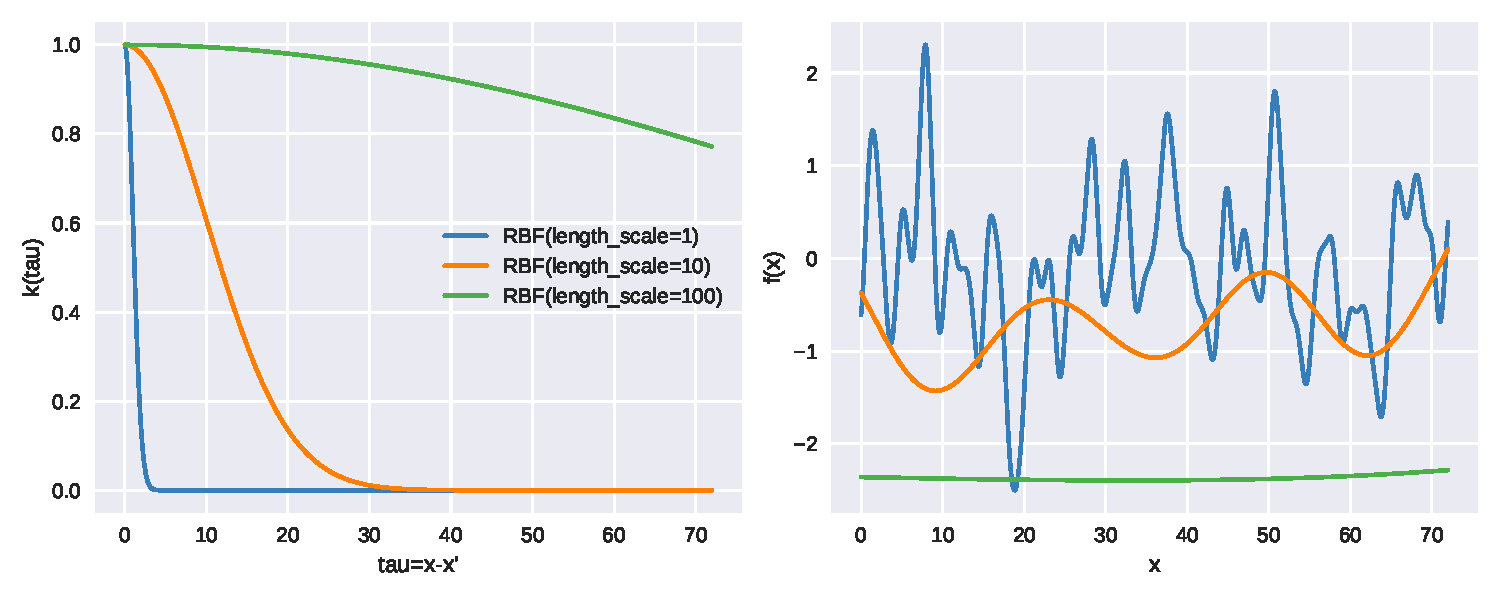
\includegraphics[width=\textwidth]{RBF_length_scale} %<< no file extension
    \caption[RBF Kernel: Kernel function wiht sample path]%<<-- Legend for the list of figures at the beginning of you thesis
   {RBF Kernel function for different length scale (left panel) and a sample
    generate by such a GP (right panel)}
    \label{fig:rbf}
\end{figure}


\subsection{The Matérn Class of Kernel Functions}

An expression for the Matérn covariance function is given by:

\begin{gather*}
    k_{\nu}(\tau) = \frac{2^{1-\nu}}{\Gamma(\nu)}(\frac{\sqrt{2\nu} \tau}{l})^{\nu} K_{\nu}
    (\frac{\sqrt{2\nu} \tau}{l})
\end{gather*}
where $\nu$ and $l$ are positive parameters and $K_{\nu}$ is a modified Bessel
function. The Matérn covariance function and corresponding sample path for different
$\nu$ are shown in figure \ref{fig:matern}.

For $\nu = r + 1/2, r \in \mathbb{N}$ the expression for the Matérn covariance
function can be simplified to:

\begin{gather}\label{kernel-matern}
    k_{\nu=r+1/2}(\tau) = \exp(-\frac{\sqrt{2r + 1} \tau}{l}) \frac{r!}{(2p)!}
    \sum_{i=0}^{r} \frac{(r+i)!}{i!(r-i)!}(\frac{2 \sqrt{2 r + 1} \tau}{l})^{r-i}
\end{gather}

\begin{figure}[!hbt]%--- Picture 'H'ere, 'B'ottom or 'T'op; '!' Try to
                    %impose your will to LaTeX
  \centering
  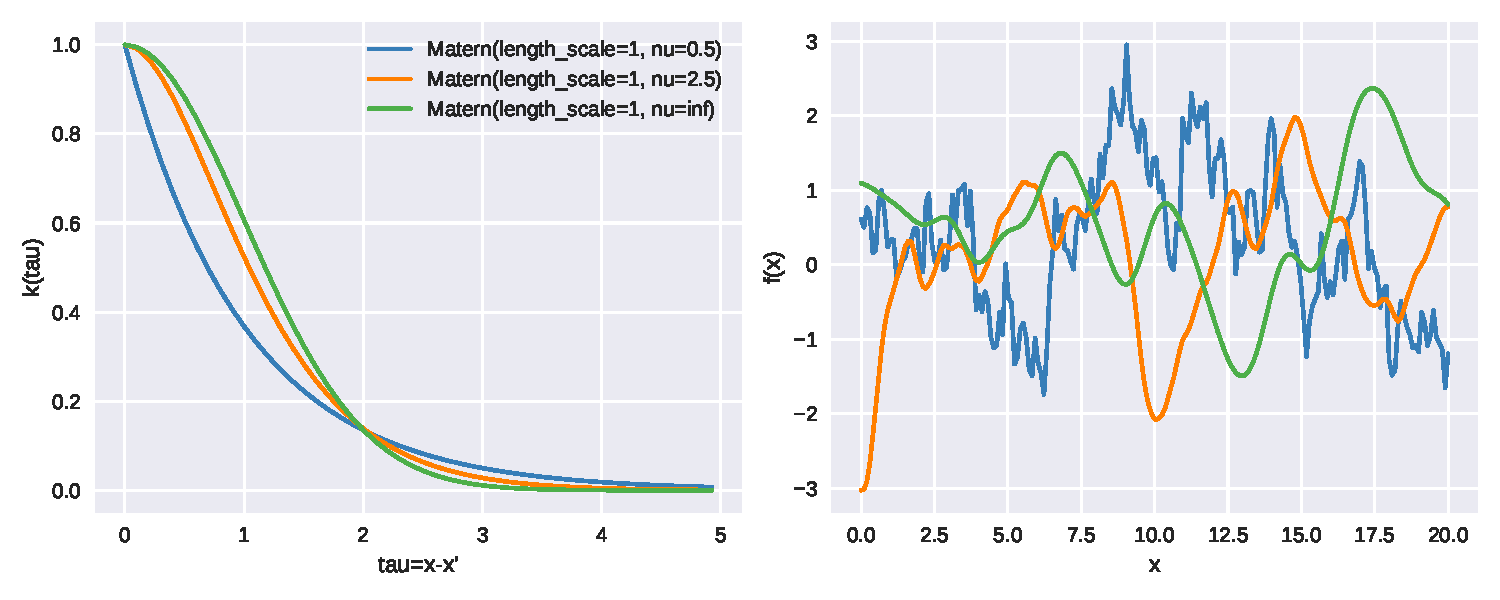
\includegraphics[width=\textwidth]{Matern_nu} %<< no file extension
  %%         --- .5\textwidth stands for 50% of text width
  \caption[Matérn Kernel: Kernel function wiht sample path]%<<-- Legend for the list of figures at the beginning of you thesis
   {Matérn kernel function for different $\nu$ (left panel) and a sample
    generate by the corresponding GP (right panel)}
  \label{fig:matern}
\end{figure}


Setting $\nu = 1/2$ with input domain $X \subset \mathbb{R}$ gives raise to a continuous-time AR(1) process,
also called Ornstein-Uhlenbeck process.
With $\nu = 1/2$, i.e. $r=0$, the Matérn covariance function is given by:
\begin{gather}\label{kernel-matern-ar1}
    k(\tau) = exp(- \tau/l)
\end{gather}
More generally, for $\nu = p - 1/2$ and $X \subset \mathbb{R}$ the Matérn kernel
matches the covariance function of a particular case of continuous AR(p) process.
For further details on this matter
see chapter 4 from the Book of \citeauthor{rasmussen_gaussian_2006}.

%and for more on the Ornstein-Uhlenbeck process see section \ref{app:ou}.

\subsection{The Periodic Kernel Function}

A periodic kernel allows to model functions that feature a repeating pattern
and has the following form:

\begin{gather*}
k(x, x') = \sigma^2 \exp(- \frac{2 \sin^2(\pi |x-x'| \backslash p)}{l^2})
\end{gather*}

where $p$ is the period, and $l$ is the length scale.
The impact of different length scales are illustrated in figure \ref{fig:periodic}.

\begin{figure}[!hbt]%--- Picture 'H'ere, 'B'ottom or 'T'op; '!' Try to
                    %impose your will to LaTeX
  \centering
  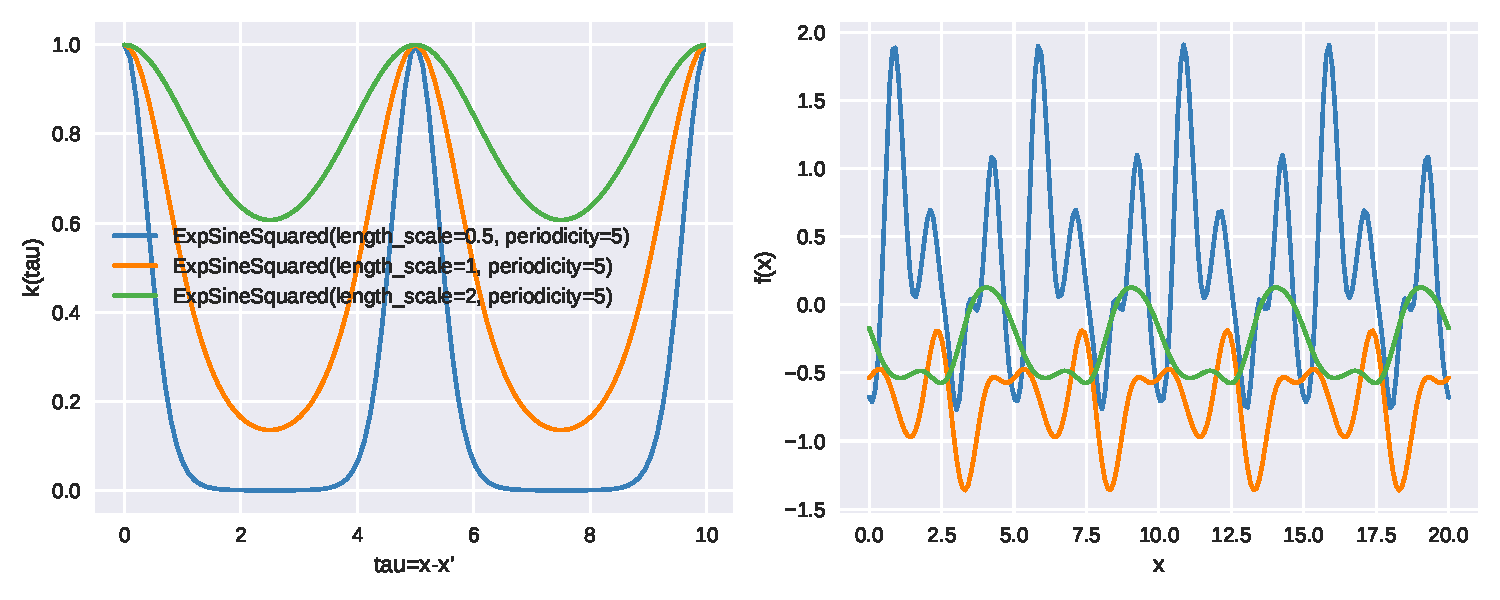
\includegraphics[width=\textwidth]{ExpSineSquared_length_scale} %<< no file extension
  %%         --- .5\textwidth stands for 50% of text width
  \caption[Periodic Kernel: Kernel function wiht sample path]%<<-- Legend for the list of figures at the beginning of you thesis
   {Periodic kernel function for different length scales (left panel) and a sample
    generate by the corresponding GP (right panel)}
  \label{fig:periodic}
\end{figure}



\subsection{Additive Kernels and Decomposition of Predictive Mean}

Additivity of the kernel implies additivity of the predictive mean.
For instance if we choose $Y(x) \sim GP(0, k(x,x'))$ with $k(x,x') = k_1(x, x') + k_2(x,x')$, then
the predictive (posterior) mean $\bar{\mu}(x^{\ast})$
is given by:
\begin{align*}
    \bar{\mu}(x^{\ast}) &= (K_{1, x^{\ast}X} + K_{2, x^{\ast}X}) (K_{XX})^{-1} \mathbf{Y}
    = K_{1, x^{\ast}X} (K_{XX})^{-1} \mathbf{Y} + K_{2, x^{\ast}X}) (K_{XX})^{-1} \mathbf{Y} \\
    &= \bar{\mu}_1(x^{\ast}) + \bar{\mu}_2(x^{\ast})
\end{align*}

where:
\begin{gather*}
    K_{1, x^{\ast}X} =
    \begin{bmatrix}
        k_1(x_1, x^{\ast}) & \dots & k_1(x_n,  x^{\ast})
    \end{bmatrix}, \\
    K_{2, x^{\ast}X} =
    \begin{bmatrix}
        k_2(x_1, x^{\ast}) & \dots & k_2(x_n,  x^{\ast})
    \end{bmatrix},
\end{gather*}
and
\begin{gather*}
        K_{XX} =
    \begin{bmatrix}
        k(x_1, x_1) & \dots & k(x_1, x_n)\\
        \vdots  &  & \vdots \\
        k(x_n, x_1) & \dots  & k(x_n, x_n)
    \end{bmatrix}
\end{gather*}

This decomposition allows us to study
the contribution of the different (additive) kernel components on the predictive mean function.


\section{Performance Assessment}\label{sec:performance-assessment}
Inference, in the case of Gaussian process regression, revolves around the posterior (predictive) distribution
of the response variable.
To evaluate how effectively the predictive distribution explains the observed values
$\mathbf{y^{\ast}}$,
it is common practice to calculate the probability of these values based on the predictive distribution.
Equation \ref{eq:posterior-gp-noise} presents an expression for the predictive distribution of
$\mathbf{Y^{\ast}}:= [Y(x_1^{\ast}), \dots, Y(x_k^{\ast})]^{\top}$ at arbitrary inputs
$X^{\ast} = [x_1^{\ast}, \dots, x_k^{\ast}]$.
Expanding the expression from \ref{eq:posterior-gp-noise} we obtain:

\begin{gather}\label{eq:predictive-dist}
    \log p(\mathbf{Y^{\ast}} = \mathbf{y^{\ast}}| \mathbf{Y}, X) =
    -\frac{k}{2} \log 2 \pi - \frac{1}{2} \log|\bar{\Sigma}| -
        \frac{1}{2}(\mathbf{y^{\ast}} - \bar{\mu})^{\top} \bar{\Sigma}^{-1} (\mathbf{y^{\ast}} - \bar{\mu})
\end{gather}
where
$\bar{\Sigma} = K_{X^{\ast}X^{\ast}} - K_{X^{\ast}X} K_{XX}^{-1} K_{XX^{\ast}}$
and $\bar{\mu} = K_{X^{\ast}X} K_{XX}^{-1} \mathbf{Y}$.

The higher the log probability, the better the fit to the data.
In contrast to other performance metrics it accounts for the complete predictive
distribution rather than just a point estimate.
For instance, when employing the sum of squared errors between the true values $y^{\ast}$ and the predictive mean
$\bar{\mu}$, the predictive covariance matrix $\bar{\Sigma}$ is completely ignored.

\section{Model Selection}

Model selection in Gaussian process regression involves identifying the optimal covariance function
along with the optimal hyperparameters.
Two common approaches for model selection are cross-validation, using a performance-based loss
function as discussed in Section \ref{sec:performance-assessment}, and Bayesian model selection,
which will be explored in the subsequent subsections.
The concepts and ideas discussed in this section are primarily derived from Chapter 5 of
the textbook from \citeauthor{rasmussen_gaussian_2006}.

\subsection{Bayesian Model Selection}

Bayesian model selection aims to find the most probable model given the available data
using a hierarchical specification of the model.
In a parametric model setting, the lowest level consists of the parameters $\beta$,
followed by the hyperparameters $\theta$, which control the parameter distribution.
The highest level encompasses the set of possible model structures $M_i$.

The posterior distribution over the parameters $\beta$ is determined using Bayes' rule:
\begin{gather*}
    p(\beta | \mathbf{Y}, X, \theta, M_i) = \frac{p( \mathbf{Y}| X, \beta,
        M_i)p(\beta|\theta, M_i)}{p(\mathbf{Y}|X, \theta, M_i)}
\end{gather*}

Here, $p(\mathbf{Y} | X, \beta, M_i)$ represents the likelihood, $p(\beta | \theta, M_i)$ denotes the prior,
and $p(\mathbf{Y} | X, \theta, M_i)$ represents the marginal likelihood.


However, in the non-parametric setting of Gaussian processes, the parameter $\beta$ does not exist and is
replaced by the function $f$ itself.
Consequently, at the lowest level, the distribution over the function $f$ is modeled using a Gaussian process.
Similarly to the parametric setting, the posterior distribution over the function values
$f^{\ast} = f(x^{\ast})$ at some arbitrary input $x^{\ast}$ is given by:
\begin{gather*}
    p(f^{\ast} | \mathbf{Y}, X, \theta, M_i) = \frac{p( \mathbf{Y}| f^{\ast}, M_i)p(f^{\ast} | \theta, M_i)}{p(\mathbf{Y}|X, \theta, M_i)}
\end{gather*}

This is equivalent to the expression in \ref{eq:posterior-gp} for the posterior distribution over the
function values $f^{\ast}$ when assuming a Gaussian process prior $f \sim GP(0, k(x,x'))$.
However, in the equation above, $k(x,x')$ is expressed through $\theta$ and $M_i$.

By assuming a prior distribution over the hyperparameters $\theta$, a similar expression can be obtained for
the posterior distribution over the hyperparameters:
\begin{gather*}
    p(\theta | \mathbf{Y}, X, M_i) = \frac{p( \mathbf{Y}| X,M_i, \theta)
        p(\theta| M_i)}{p(\mathbf{Y}|X, M_i)}
\end{gather*}
Maximizing $p(\theta | \mathbf{Y}, X, M_i)$ yields the optimal hyperparameters.
However, when non-Gaussian priors are assumed for $\theta$, evaluating $p(\theta | \mathbf{Y}, X, M_i)$
can be challenging.
In such cases, it is common to maximize the marginal likelihood $p(\mathbf{Y} | X, \theta, M_i)$
with respect to the hyperparameters $\theta$.
This approach is equivalent to assuming uniform distributions over the hyperparameters.
The next subsection will provide more details on how to calculate and maximize the
marginal likelihood for Gaussian process regression.

Note that the scheme mentioned above can be extended to maximize the posterior over the model structures
$M_i$ in order to determine the optimal model structure.
In Gaussian process regression, this corresponds to finding the optimal kernel function type.
However, instead of directly evaluating the posterior, it is often achieved through simultaneous optimization of
the marginal likelihood with respect to the model structure $M_i$ and its hyperparameters $\theta$.
By jointly optimizing these components, we can effectively identify the most suitable kernel function for
the given problem.



%The posterior distribution over the model $M_i$ is given by:
%\begin{gather*}
%    p(M_i | \mathbf{Y}, X) = \frac{p( \mathbf{Y}| X)
%        p(M_i)}{p(\mathbf{Y}|X)}
%\end{gather*}
%where $p(\mathbf{Y}|X) = \sum_i p(\mathbf{Y}|X, M_i)p(M_i)$


\subsubsection{Marginal Likelihood}

In the context of Bayesian linear regression, the marginal likelihood expression was previously
introduced in subsection \ref{subsec:bayesian-linear-regression},
assuming a prior distribution of $p(\beta) = \mathcal{N}(0, \Sigma_p)$ and a likelihood function of
$p(\mathbf{Y} | X, \beta) = \mathcal{N}(X \beta, \Sigma_r)$.
The following expression for the marginal likelihood is obtained by marginalizing over $\beta$:

\begin{gather}\label{eq:marginal-likelihood2}
    p(\mathbf{Y}|X) = \int p(\mathbf{Y}|X,\beta) p(\beta) d\beta = \N(0, X \Sigma_p X^{\top} + \Sigma_r)
\end{gather}

Furthermore, as discussed in section \ref{sec:gaussian-process-regression},
the marginal likelihood can also be represented as a distribution over the function $Y(x)$:
\begin{gather*}
    Y(x) \sim GP(0, k(x, x'))
\end{gather*}
Here, the kernel function $k(x, x')$ is chosen such that for an index set $X$,
we obtain $K_{XX} = X \Sigma_p X^{\top} + \Sigma_r$.

By the definition of a Gaussian process, $\mathbf{Y}|X$ follows a multivariate normal distribution
with a covariance matrix of $K_{XX}(\theta)$, which is a function of the hyperparameters $\theta$.
The log marginal likelihood is hence given by:
\begin{gather}\label{eq:gaussian-marginal-likelihood}
    \log p(\mathbf{Y} | X, \theta) = - \frac{1}{2} \mathbf{Y}^{\top} K_{XX}^{-1}(\theta) \mathbf{Y} -
    \frac{1}{2} \log |K_{XX}(\theta)| - \frac{n}{2} \log 2 \pi
\end{gather}

Since the marginal likelihood already incorporates a trade-off between model fit and
model complexity, it is a suitable candidate for solving the model selection problem.
The first term, $- \frac{1}{2} \mathbf{Y}^{\top} K_{XX}^{-1}(\theta) \mathbf{Y}$,
represents a measure of the data fit. The second term, $\frac{1}{2} \log |K_{XX}(\theta)|$,
penalizes more complex models. The last term $\frac{n}{2} \log 2 \pi$ serves as a normalization constant.
















\chapter{Methods}\label{ch:methods}

The last chapter introduced Gaussian process regression to establish a mapping
between a time point $x$ and its corresponding BP value. Since Gaussian Processes
are capable of modeling time series in continuous time and hence deal with
irregularly spaced data, they seem to be a good candidate for modeling a time
series from which we only have irregularly sampled noisy measurements.

This chapter outlines the methodology for evaluating the performance of Gaussian
process regression and baseline methods for estimating blood pressure values from
noisy measurements. It also discusses the analysis of adversarial factors that may
affect estimation accuracy.


%Additionally, the impact of different adversarial factors on the target measure
%estimate should be investigated. This will be described in section
%\ref{sec:adversarial-analysis}.



\section{Problem Statement}

Recall the problem statement from section \ref{sec:problem-statement}. First, we
assumed the following model for the BP measurements $Y(x)$ at a time point $x$:

\begin{align*}
    Y(x) = f(x) + \epsilon && \epsilon \sim \N(0, \sigma_n^{2})
\end{align*}

where $f(x)$ denotes the true BP process and $\epsilon$ is iid measurement noise,
independent from $f(x)$.

The goal is to estimate the true BP values $f(x)$ at some input time $X$,
based on noisy observations of $f(x)$ at some training time points $X_{train}$.
For the sections of this chapter, we define:

\begin{itemize}
    \item $X := \{ x_1, \dots, x_n \}$: An index set spanning the one-week time
    range of interest, with 10 BP values per hour.
    It defines the time points at
    which we want to predict BP values and hence represents the regression input.

    \item $X_{train} \subset X$: The training indexes. \\

    \item $G_X := (g(x) : x \in X )$ for some function $g(x)$.
    Specifically:
    \begin{description}
        \item $F_X := (f(x) : x \in X)$: The true BP values at inputs $X$.
        \item $Y_X = (Y(x) : x \in X)$: The noisy BP measurements at inputs $X$,
        which constitute the response variable in the context of regression.
        \item $Y_{X_{\text{train}}} := (Y(x) : x \in X_{\text{train}})$: The noisy
        measurements at training indexes.
    \end{description}

%    \item $\text{ }$\\

    \item $(X_{train}, Y_{X_{train}})$: The training data used for estimating $F_X$


%    \item $\text{ }$\\

    \item $K_{XX'} := \begin{bmatrix}
            k(x_1, x'_1) & \dots & k(x_1, x'_m)\\
            \vdots  &  & \vdots \\
            k(x_n, x'_1) & \dots  & k(x_n, x'_m)
         \end{bmatrix}$ ,for some kernel function, $k(x, x')$ \\

        and some inputs $X=(x_1, \dots x_n)$ and $X'=(x'_1, \dots x'_m)$.
%    \item $\text{ }$\\
\end{itemize}

Additionally, when referring to the estimated values,
$\hat{F}_X$ is used instead of $F_X$.


\section{Overview}

To assess the suitability of GPs for this problem, the following tasks have been defined:
\begin{itemize}
    \item Simulate $F_X$ and the training data ($X_{train}$, $Y_{X_{train}}$)
    (section \ref{sec:blood-pressure-time-series-simulation})
    \item Employ Gaussian process regression to obtain $\hat{F}_X$ from the training data
     (section \ref{sec:evaluation-gaussian-process-regression})
    \item Derive target measures from $\hat{F}_X$, including 95\% credible intervals (section \ref{sec:target-measures})
    \item Evaluate performance using:
    \begin{itemize}
        \item CiCoverage: Equals one if the true target measure value extracted from $F_X$ was
        covered by the credible interval, zero otherwise.
        \item CiWidth: The width of the credible interval
    \end{itemize}
\end{itemize}
These steps are repeated $S=100$ times, and the final performance is assessed by averaging CiCoverage and CiWidth.
Pseudocode \ref{pc:simulation-evaluation-flow} provides a more detailed illustration of this process.

To contextualize the performance of GP regression, it is compared to the performance of
baseline methods (section \ref{sec:baseline-methods}).
Additionally, the impact of adversarial factors on estimation accuracy is discussed in section \ref{sec:adversarial-analysis}.

\section{Target Measures}\label{sec:target-measures}

In subsection \ref{subsec:target-measures}, the mean BP over different time
windows and TTR has been defined as the measures of interest. These measures
are extracted from $F_X$ to obtain the true target measure values and
from $\hat{F}_X$ to obtain the estimated target measures.

The \textbf{one-week mean BP}, $\bar{F}_X$, was calculated as the mean of all values in
$F_X$:
\begin{gather*}
    \bar{F}_{X} = \frac{1}{n} \sum_{x \in X} f(x)
\end{gather*}

The \textbf{one-hour and one-day BP means}, $\bar{F}_{X_1} \dots \bar{F}_{X_W}$,
were calculated by taking the mean value of $f(x)$ evaluated at the different
time windows $X_1 \dots X_W \subset X$.
For the first one-hour or one-day window $X_1$, this is:
\begin{gather*}
    \bar{F}_{X_1} = \frac{1}{n_1} \sum_{x \in X_1} f(x), \\
    \text{with $n_1$ being the number of elements in $X_1$}
\end{gather*}

To obtain a single measure,
in each simulation iteration $s$, a time window
was chosen uniformly at random from $X_1 \dots X_W$.
The estimation performance was assessed for this time window only, and
the mean performance over all $S$ simulations was reported.

\textbf{TTR} was calculated by dividing the number of BP values in $F_X$
within the target range by the total number of values in $F_X$:
\begin{gather*}
    \frac{1}{n} \sum_{x \in X} \mathbbm{1}\{\ 90 < f(x) < 125 \}
\end{gather*}


\section{Blood Pressure Time Series Simulation}\label{sec:blood-pressure-time-series-simulation}

For simulating the blood pressure time series, the goal is to match the
properties described in section \ref{sec:problem-statement}. Simulation starts by
generating the true BP time series process, $f(x)$. This process is then sampled
at the desired time points $X$ to obtain $F_X$. Finally, noise is added to obtain
$Y_X$.

The true BP process $f(x)$ is modeled by a Gaussian process (true GP)
since GPs are flexible enough to represent the properties
specified for $f(x)$ in section \ref{sec:characteristics-of-the-blood-pressure-time-series}.

\subsection{Mean function}
A reasonable assumption for the mean function is to keep it constant and
equal to the global mean BP value of 120 mmHg. We have:
\begin{gather*}
    f(x) \sim GP(120, k(x,x'))
\end{gather*}

From section \ref{subsec:mean-function}, we know that this is the same as writing:
\begin{gather*}
    f(x) - 120 \sim GP(0, k(x,x'))
\end{gather*}
For simplicity, we are going to completely ignore this constant
mean function throughout the rest of the thesis and
model the true BP process $f(x)$ with the following GP:
\begin{gather*}
    f(x) \sim GP(0, k(x,x'))
\end{gather*}
where we write $f(x)$, although we actually mean $f(x) - 120$.


\subsection{Kernel function}
The chosen kernel function to match the properties from
section \ref{sec:characteristics-of-the-blood-pressure-time-series} is:
\begin{gather*}\label{def:true_gp}
k(x, x') = 2.24^{2} * \text{Matérn}(l=3, \nu=0.5) +
14^{2} * \text{Periodic}(l=3, p=24) +  2.24^{2} * \text{RBF}(l=50)
\end{gather*}
where $l$ denotes the length scale, and $p$ denotes the periodicity
of the corresponding kernel function in hours.
The formal definition of the Matérn, Periodic, and RBF kernel
functions and their parameters is provided in section \ref{sec:kernel}.

Each of these kernels models one of the components described in
\ref{sec:characteristics-of-the-blood-pressure-time-series}:
\begin{itemize}
    \item The Matérn kernel with $\nu=0.5$ models the AR(1) component
    \item The Periodic kernel models the circadian cycle
    \item The RBF kernel models a long-term trend
\end{itemize}

The kernel function is illustrated in figure \ref{fig:true_kernel}, and
some samples drawn from this GP are shown in Figure \ref{fig:true_gp_samples}.

\begin{figure}[!ht]
    \centering
    \includegraphics[width=0.6\linewidth]{Pictures/plots_final/sin_rbf_default_0.2/09_06_09_09_17/plot_kernel_true}
    \caption{The true kernel function $k(x,x')$}
    \label{fig:true_kernel}
\end{figure}

\begin{figure}[!ht]
\centering
\begin{subfigure}{.45\textwidth}
    \centering
    \includegraphics[width=\linewidth]{Pictures/plots_final/sin_rbf_default_0.05/09_06_08_59_46/plot_true_mean_decomposed}
    \includegraphics[width=\linewidth]{Pictures/plots_final/sin_rbf_default_0.05/09_06_09_00_31/plot_true_mean_decomposed}
    \includegraphics[width=\linewidth]{Pictures/plots_final/sin_rbf_default_0.05/09_06_09_00_58/plot_true_mean_decomposed}
  \caption{The sample $F_X$ shown to the right, decomposed in to the contribution of the Periodic kernel (orange),
      Matérn kernel (blue), RBF kernel (green).}
  \label{fig:true_mean_decomposed}
\end{subfigure}\hfill
\begin{subfigure}{.45\textwidth}
    \centering
    \includegraphics[width=\linewidth]{Pictures/plots_final/sin_rbf_default_0.05/09_06_08_59_46/plot_true_with_samples}
    \includegraphics[width=\linewidth]{Pictures/plots_final/sin_rbf_default_0.05/09_06_09_00_31/plot_true_with_samples}
    \includegraphics[width=\linewidth]{Pictures/plots_final/sin_rbf_default_0.05/09_06_09_00_58/plot_true_with_samples}
  \caption{Each figure shows one sample $F_X$ drawn from the true GP (red dashed line) with noisy observations
      (red dots) sampled at a frequency of 0.5/hour}
  \label{fig:sub2}
\end{subfigure}
\caption{Three samples (right side) drawn from the true GP and the decomposition of theses samples (left side)}
\label{fig:true_gp_samples}
\end{figure}


\subsection{Simulation of the BP Measurements}\label{subsec:simulation-of-the-bp-measurements}

The BP measurements time series process $Y(x)$ is obtained by adding iid measurement noise
$\epsilon \sim \N(0, \sigma_n^2)$ to $f(x)$.
The measurement noise variance
$\sigma_n^2$ is set to 31 mmHg², as explained in subsection
\ref{sec:characteristics-of-the-blood-pressure-time-series}.
The measurement indexes $X_{train}$ are then chosen
from $X$, yielding the training data, $Y_{X_{train}}$.
The different downsampling patterns used to produce the training data
are described in section \ref{sec:adversarial-analysis}.

Appendix \ref{sec:properties-of-the-simulated-time-series-samples} additionally presents
the distributions of some simulated BP measurement properties.


\section{Gaussian Process Regression}\label{sec:evaluation-gaussian-process-regression}

A Gaussian process regression was fitted to $Y_{X_{\text{train}}}$ to estimate $F_X$.
The kernel function used has the same form as the one used for simulation
but with variable hyperparameters:

\begin{gather*}\label{def:gp_fit}
    k(x, x') = \sigma_M^2 \cdot \text{Matérn}(l, \nu=0.5) +
               \sigma_P^2 \cdot \text{Periodic}(l, p=24) +
               \sigma_R^2 \cdot \text{RBF}(l)
\end{gather*}

The hyperparameters, $\sigma_M^2$, $\sigma_P^2$, $\sigma_R^2$, and $l$, were found by
maximizing the marginal likelihood, as described in subsection
\ref{subsec:marginal-likelihood}, yielding the optimal kernel $\hat{k}(x, x')$.

From $\hat{k}(x, x')$, the predictive distribution over $F_X$ was calculated.
Furthermore, the target measures, including credible intervals, were estimated by
sampling from the predictive distribution.
Pseudocode \ref{pc:simulation-evaluation-flow} describes the entire simulation flow
for evaluating the performance of GP regression for a specific target measure.


\begin{algorithm}[h!] \caption{Simulation and Evaluation Flow}
 \hspace*{\algorithmicindent} \textbf{Inputs:} \\
 \hspace*{\algorithmicindent} $X$ \algorithmiccomment{The regression input} \\
 \hspace*{\algorithmicindent} $K_{XX}$ \algorithmiccomment{ The true kernel function evaluated at the input $X$}\\
 \hspace*{\algorithmicindent} TargetMeasure \algorithmiccomment{Function to extract target measure from $F_X$ or $\hat{F}_X$} \\
 \hspace*{\algorithmicindent} \textbf{Output:} \\
 \hspace*{\algorithmicindent} CiCoverage \algorithmiccomment{Credible interval coverage}\\
 \hspace*{\algorithmicindent} CiWidth \algorithmiccomment{Credible interval width}\\
\begin{algorithmic}[1]
    \State \textbf{Initialize:} CiCoverageList = $\left[ \text{ } \right]$, CiWidthList = $\left[ \text{ } \right]$,
    \For {$s = 0$ \dots $S$}
        \State $F_X =$ sample from $\N(0, K_{XX})$ \algorithmiccomment{Sample from the true GP}
        \State $X_{train} \subset X$ \algorithmiccomment{Choose training indexes}
        \State $Y_{X_{train}} = F_{X_{train}} + \epsilon$, $\epsilon \sim  \N(0, \sigma_n^2)$
        \State $\hat{k}(x,x')=$ GP.fit($X_{train}, Y_{X_{train}}$) \algorithmiccomment{Find the optimal kernel}
        \State $\hat{F}_X = \hat{K}_{XX_{train}} (\hat{K}_{X_{train}X_{train}} + \sigma_n^2 I)^{-1} Y_{train}$ \algorithmiccomment{predictive mean}
        \State $\hat{\Sigma}_{F_X} = \hat{K}_{XX} -\hat{K}_{XX_{train}}(\hat{K}_{X_{train}X_{train}} + \sigma_n^2 I)^{-1}\hat{K}_{X_{train}X}$ \algorithmiccomment{predictive covariance}
        \State \textbf{Initialize:} $\hat{M} = \left[ \text{ } \right]$
        \For {$k = 0$ \dots $K$}
            \State $\hat{F}_{X,k} = $ sample from $\N(\hat{F}_X, \hat{\Sigma}_{F_X} )$ \algorithmiccomment{Sample from predictive distribution}
            \State $\hat{M}$.append(TargetMeasure($\hat{F}_{X, k}$)) \algorithmiccomment{Extract target measure}
        \EndFor
    \State $m =$ TargetMeasure($F_X$) \algorithmiccomment{Extract true target measure}
    \State $\hat{m} = $mean($\hat{M}$)
    \State $ci = (\text{quantile}_{\alpha/2}, \text{quantile}_{1-\alpha/2}$) \algorithmiccomment{Equal-tailed credible interval}
    \State CiCoverageList.append($ ci\left[ 0 \right] \leq m \leq ci\left[ 1 \right]$)
    \State CiWidthList.append($ci\left[ 1 \right] - ci\left[ 0 \right] $)
    \EndFor
    \State CiCoverage = mean(CiCoverageList)
    \State CiWidth = mean(CiWidthList)
\end{algorithmic}
\end{algorithm}\label{pc:simulation-evaluation-flow}



%	Calculate TTR:
%	\begin{itemize}
%			\item General: Number of predicted data points within the range over the total number of data points
%			\item Naive TTR: Number of available data points within the range over the total number of available data points
%			\item True: $\sum_{i=1}^{n} \mathbbm{1}\{\ f(x_i) < \gamma \}$.
%			\item GP/Spline/: $\sum_{i=1}^{n} \mathbbm{1}\{\ \bar{\mu}_i < \gamma \}$. Sample from Posterior to get CI
%			\item Naive: $\sum_{i=1, y_i \in y_{train}}^{m} \mathbbm{1}\{\ y_i < \gamma \}$
%	\end{itemize}



%$F_X$ is replaced by $\hat{F}_X$ for extracting the measures from the
%estimated BP values.

%
%Simulation of true BP signal and measurements:
%    \begin{itemize}
%        \item $X=\{x_1, \dots x_n\}$: The time points of interest, which is one week of data with 10 BP values per hour.
%        \item $f_X := \{f(x_1) \dots f(x_n)\}$: The true BP signal $f(x)$ drawn from $GP(0, k_{true}(x,x'))$ evaluated at inputs $X$.
%        \item $y_X := \{y(x_1) \dots y(x_n)\}$: The noisy BP measurements. $y(x)= f(x) + \epsilon$ with $\epsilon \sim N(0, \sigma_n^2)$
%    \end{itemize}
%
%Based on subsampling scheme choose $X_{train} \subset X$ with $|X_{train}| = m$ and $X_{test} = X \setminus X_{train}$.
%\begin{itemize}
%    \item $y_{train} := \{y(x_i) | x_i \in X_{train}\}$
%    \item  $f_{train} := \{f(x_i) | x_i \in X_{train}\}$
%\end{itemize}
%
%
%	Fit GP regression model to training data $y_{train}$, $X_{train}$:
%    \begin{itemize}
%        \item $k_{fit}$: The fitted kernel function with hyperparameters $\theta$ that maximizes the marginal likelihood
%        $p(y_{train}| \theta)$
%        \item $p(f_X| y_{train}, k_{fit}) = N(\bar{\mu}, \bar{\Sigma})$:
%        The posterior (predictive) probability density of $f_X$. The posterior mean vector
%        $\bar{\mu} \in \mathbb{R}^n$ contains the point estimates for $f_X$.
%        \begin{itemize}
%            \item $\bar{\mu}_{train} := \{\bar{\mu}_i | x_i \in X_{train}\}$
%            \item $\bar{\Sigma}_{train} := \bar{\Sigma}_{i,j}$ where $\{i | x_i \in X_{train}\}$ and $\{j | x_j \in X_{train}\}$
%
%        \end{itemize}
%    \end{itemize}
%
%	Output of GP Regression are predictive probabilities $p(f_{train}| y_{train})$,
%		$p(f_{test}| y_{train})$ and $p(f_{X}| y_{train})$:
%			\begin{itemize}
%				\item Note $\bar{\mu}_{train} \neq f_{train}$ due to the measurement error. \\ If
%				$f_{train}$ was known: $p(f_{train}| f_{train}, GP_{fit}) = N(\bar{\mu}_{X_{train}},
%				\bar{\Sigma}_{X_{train}})$
%				with $\bar{\mu}_{train} = f_{train}$ and $\bar{\Sigma}_{train} = {\displaystyle O}$
%			\end{itemize}
%


\section{Baseline Methods}\label{sec:baseline-methods}

Some other methods were fitted to $Y_{X_{train}}$ as a reference, to which
the GP performance was compared to.
The chosen baseline methods presented in this section are: linear regression,
smoothing spline, overall mean, and naive TTR.
All methods, but naive TTR, estimate the target measure through the estimation of $F_X$.
The calculation of the target measure and confidence interval is described in
Pseudocode \ref{pc:target-measure-baseline}.
The procedure is equivalent to GP regression, except that one does not sample from
the posterior distribution but uses bootstrap samples instead.


\begin{algorithm}[!ht] \caption{Target Measrue Estimation with CI}
 \hspace*{\algorithmicindent} \textbf{Inputs:} \\
 \hspace*{\algorithmicindent} $X$ \algorithmiccomment{The regression input} \\
 \hspace*{\algorithmicindent} $F_X$  \algorithmiccomment{True BP values at inputs $X$} \\
 \hspace*{\algorithmicindent} $X_{train}, Y_{X_{train}}$ \algorithmiccomment{The training data} \\
 \hspace*{\algorithmicindent} RegressionMethod \algorithmiccomment{The baseline method} \\
 \hspace*{\algorithmicindent} TargetMeasure \algorithmiccomment{Function to extract target measure from $F_X$ or $\hat{F}_X$} \\
 \hspace*{\algorithmicindent} \textbf{Output:} \\
 \hspace*{\algorithmicindent} CiCoverage \algorithmiccomment{Credible interval coverage}\\
 \hspace*{\algorithmicindent} CiWidth \algorithmiccomment{Credible interval width}\\
\begin{algorithmic}[1]
    \State \textbf{Initialize:} $\hat{M} = \left[ \text{ } \right]$
    \For {$k = 0$ \dots $K$} \algorithmiccomment{K bootstrap iterations}
        \State $X^{\ast} = $ sample with replacement from $X_{train}$
        \State $\hat{F}_{X,k} = $ RegressionMethod.fit($X^{\ast}, Y_{X^{\ast}}$).predict($X$)
        \State $\hat{M}$.append(TargetMeasure($\hat{F}_{X, k}$)) \algorithmiccomment{Extract target measure}
    \EndFor
    \State $m =$ TargetMeasure($F_X$) \algorithmiccomment{Extract true target measure}
    \State $\hat{m} = $mean($\hat{M}$)
    \State $ci = ((2\hat{m} - \text{quantile}_{1-\alpha/2}(\hat{M}), (2\hat{m} - \text{quantile}_{\alpha/2}(\hat{M})))$ \algorithmiccomment{Confidence interval}
    \State CiCoverage = ($ ci\left[ 0 \right] \leq m \leq ci\left[ 1 \right]$)
    \State CiWidth = ($ci\left[ 1 \right] - ci\left[ 0 \right] $)
\end{algorithmic}
\end{algorithm}\label{pc:target-measure-baseline}




\subsection{Linear Regression}

The model used has already been presented in section \ref{sec:linear-regression} and
it features a linear trend and seasonal component:
\begin{gather*}
Y(x) = \beta_0 + \beta_1 x + \beta_2 \cos(2 \pi f x) + \beta_3 \sin(2 \pi f x) + R(t), \\
\end{gather*}
where $f$, the frequency, is known and equals $1/\text{period} = 1/24$.

The seasonal component has variable phase shift and amplitude.
Ordinary least square regression has been fit to the training data
$(X_{train}, Y_{X_{train}})$ to obtain the regression coefficients and thus
$\hat{F}_X$.
%Figure \ref{fig:post-linear} shows how an example of $\hat{F}_X$ estimated
%using training data.
%

\subsection{Smoothing Spline}
The scikit-learn Python package has been used to
generate smoothing splines for predicting $F_X$.
First, $X_{train}$ and $X$ were transformed to cubic B-splines using the \\
"sklearn.preprocessing.SplineTransformer" class.
Knots have been placed uniformly along the quantiles of $X_{train}$.
Ordinary least square regression is then fit to the transformed training
input $X\text{trans}_{train}$ and the response $Y_{X_{train}}$.
The number of knots determines the smoothness of the resulting function,
and the optimal number has been identified through 10-fold
cross-validation. The
%
The code section \ref{code:smoothing-spline} provides more implementation details,
and figure \ref{fig:post-spline} shows an example of $\hat{F}_X$ estimated
from training data using smoothing splines.

%
\begin{figure}[!ht]
\centering

\begin{minted}[frame=single]{python}
    import numpy as np
    from sklearn.preprocessing import SplineTransformer
    from sklearn.linear_model import LinearRegression

    def fit_and_predict_smoothing_spline(
                    X_train: np.ndarray,Y_X_train: np.ndarray, X: np.ndarray,
                    n_knots: int) -> np.ndarray:
        """
        Parameters
        ----------
        X_train, Y_X_train: The training data
        X: The time indexes at which to generate predictions
        n_knots : Number of knots of the splines

        Returns
        ---------
        F_X_hat: The BP value predictions at inputs X
        """

        spline = SplineTransformer(degree=3, n_knots=n_knots,
                                   extrapolation="constant",
                                   knots="quantile")
        # Compute knot positions of splines.
        spline.fit(X_train)
        # Transform to B-splines
        Xtrans_train = spline.transform(X_train)
        Xtrans = spline.transform(X)

        # Fit a linear regression
        lm = LinearRegression(fit_intercept=False).fit(Xtrans_train, Y_X_train)

        # Predict BP values at inputs X
        F_X_hat = lm.predict(Xtrans)
        return F_X_hat

\end{minted}
\captionof{listing}{Smooting Spline Estimation of $F_X$}
\end{figure} \label{code:smoothing-spline}



\begin{figure}[!ht]
\centering
\begin{subfigure}{.5\textwidth}
    \centering
    \includegraphics[width=\linewidth]{
        Pictures/plots_final4/sin_rbf_default_0.2/09_12_13_05_43/plot_posterior_confint_linear}
    \caption{Linear Regression}
    \label{fig:post-linear}
\end{subfigure}\hfill
\begin{subfigure}{.5\textwidth}
    \centering
    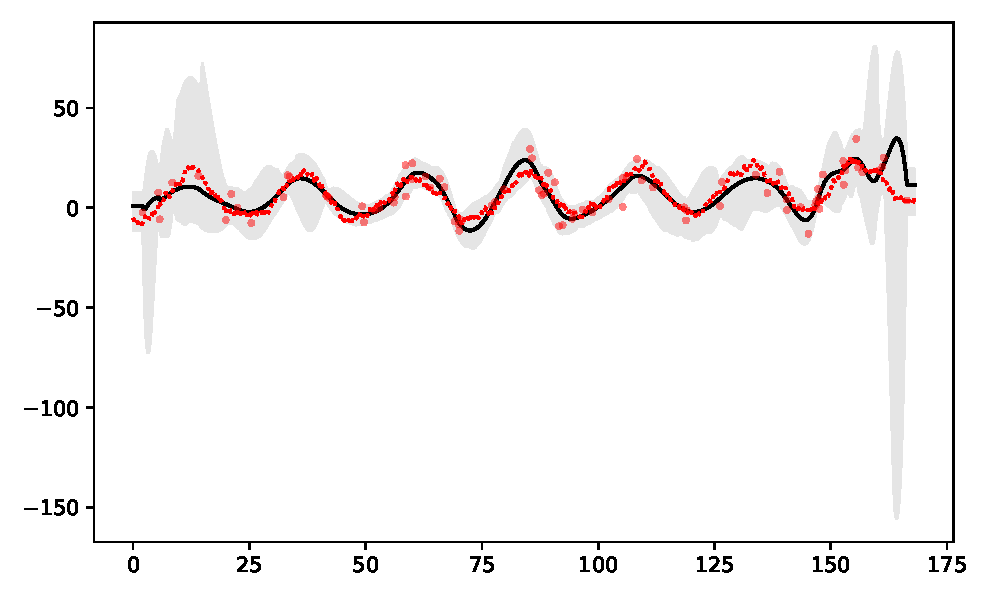
\includegraphics[width=\linewidth]{
        Pictures/plots_final4/sin_rbf_default_0.2/09_12_13_05_43/plot_posterior_confint_spline}
    \caption{Smoothing Spline}
    \label{fig:post-spline}
\end{subfigure}
\caption{Linear Regression and Smoothing spline used
to estimate some example of true BP values $F_X$. The estimated BP values $\hat{F}_X$ (black line), the
        true BP values (red dashed line) and the training data (red dots). The gray area shows
the bootstrap CI.}
\label{fig:regression-example}
\end{figure}


\subsection{Overall Mean}
This method sets $\hat{F}_X$ to the mean of all measurements
$Y_{X_{train}}$ everywhere.


\subsection{Naive TTR}
This method directly estimates the target measures
from the noisy measurements $Y_{X_{train}}$, without estimating $F_X$
first.
The one-hour, one-day, and one-week means were calculated by
taking the mean of the available measurements within the time period.
If no measurements are available within that period, the mean
overall measurements were used.

For calculating TTR, the number of measurements within the range over
the total number of available data points.


\section{Adversarial Analysis}\label{sec:adversarial-analysis}

This section explores the influence of the sampling pattern on the accuracy of
target measure estimates.
As discussed in Section \ref{sec:characteristics-of-the-blood-pressure-time-series},
data density was expected to vary within the Aktiia population,
and measurements were not uniformly sampled.
Instead, data density followed a circadian cycle, referred to as "seasonal sampling."

To create varying levels of data density, downsampling was applied to the dataset
$X$ to obtain $X_{train}$.
Different downsampling factors were investigated, including 20, 10, 5, and 2.5.
A downsampling factor of 20 indicated that $X_{train}$ contained only
5\% of the original data in $X$, which initially had 10 time points per hour.
Consequently, a downsampling factor of 20 or a data fraction of 0.05 implied
that measurements were, on average, taken every other hour.

Seasonal sampling was implemented by extracting the true seasonal component
from the original BP samples. The values of these seasonal components
shifted to contain only positive values and scale to sum up to one,
served as probability weights when selecting data for $X_{train}$ from $X$.
A more extreme seasonal sampling pattern has been produced by
using the squared values of the seasonal component as probability weights.
The decomposed seasonal component and the resulting seasonal sampling are
illustrated in Figure \ref{fig:seasonal-sampling}.




%Finally, we want to study the impact of the sampling pattern on the
%target measure estimates.
%As described in section \ref{sec:characteristics-of-the-blood-pressure-time-series},
%the data density is expected to vary within the Aktiia population, and
%measurements might
%also not be sampled uniformly, but data density might follow the circadian cycle.
%We will refer to the latter phenomenon as seasonal sampling.
%
%Different degree of data density was produced by downsampling
%$X$ to obtain $X_{train}$. The different downsampling factors studied
%are: 20, 10, 5 and 2.5.
%A downsampling factor of 20 implies that $X_{train}$
%contains a fraction of 0.05 of the original data $X$, which contains
%10 time points per hour. A downsampling factor of 20 and a data fraction of
%0.05 therefore implies that measurements have on average been
%taken every other hour.
%
%Seasonal sampling was achieved by extracting the true seasonal component from
%the true BP sample. The values of the seasonal components were used
%as probability weights when choosing $X_{train}$ from $X$. The decomposed
%seasonal component and the resulting seasonal sampling are illustrated
%in figure \ref{fig:seasonal-sampling}.
%

\begin{figure}[!ht]
\centering
\begin{subfigure}{.3\textwidth}
    \centering
    \includegraphics[width=\linewidth]{
        Pictures/plots_final4/sin_rbf_seasonal_default_0.2/09_12_13_15_56/plot_true_mean_decomposed}
    \caption{Decomposed $f(x)$}
%    \label{fig:post-linear}
\end{subfigure}\hfill
\begin{subfigure}{.3\textwidth}
    \centering
    \includegraphics[width=\linewidth]{
        Pictures/plots_final4/sin_rbf_seasonal_default_0.2/09_12_13_15_56/plot_true_with_samples}
    \caption{$f(x)$ and measurments from seasonal sampling.}
%    \label{fig:post-spline}
\end{subfigure}\hfill
\begin{subfigure}{.3\textwidth}
    \centering
    \includegraphics[width=\linewidth]{
        Pictures/plots_final4/sin_rbf_seasonal_extreme_0.2/09_13_07_48_30/plot_true_with_samples}
    \caption{$f(x)$ and measurments from extreme seasonal sampling.}
%    \label{fig:post-linear}
\end{subfigure}
\caption{Panel (b) and (c) show the sample $f(x)$ (red dashed line) drawn from the true GP with measurments generated
by seasonal and extreme sampling (red dots). Panel (a) shows $f(x)$ decomposed into its components.
The probability weights used for downsamplin $X$ are calculated
from the values of the periodic component (orange)}
\label{fig:seasonal-sampling}
\end{figure}



\section{Computational Frameworks}

All code has been written in Python.
For Gaussian process simulation and regression, for fitting the Smoothing Spline
and Linear Regression, the Pyton package scikit-learn
has been used.

%Unless otherwise stated the Pyton package scikit-learn has been used.














\chapter{Results}\label{ch:results}





\chapter{Discussion and Conclusion}\label{ch:discussion-and-conclusion}

\subsection{Comparison of GP Regression and Baseline Methods}

Overall, when considering different downsampling patterns and target measures,
GP regression outperforms the baseline methods. This superiority is particularly
evident when calculating the mean over small time windows, such as one-hour and one-day means.
This performance can be attributed to the fact that GP regression explicitly models
the dependencies among BP values across different time points. Consequently,
the uncertainty predictions are based on the amount of data available at time
points that are highly correlated, either positively or negatively, with the time
point of prediction.
Since the degree of correlation depends on the proximity to the prediction point,
this results in larger CI when data density is low around the prediction point.

Linear regression, on the other hand, provides the narrowest CIs and maintains adequate
CI coverage for the one-week mean under large downsampling factors. However,
linear regression does not exhibit significant improvement with an increase in data.
This can be attributed to the inherent
limitations of the linear model, which can only capture a linear trend with a perfect sinusoidal
seasonal pattern. This characteristic makes the method less reliant on the amount of data available.

In contrast, spline regression is a non-parametric method and is thus more data-dependent.
Spline regression does not yield meaningful results under large downsampling factors,
except when estimating TTR, where the locally unstable BP estimates have a relatively smaller impact.
For the same reason, spline regression does not attempt to fit a cyclic pattern and therefore struggles with seasonal sampling.

Although GPs fall under the category of non-parametric methods, they offer the option to express
prior beliefs about the function of interest through the choice of kernel.
In our case, a function with a cyclic pattern with a periodicity of 24 hours, an AR component, and a long-term trend are favored.
This choice does not impose as many constraints on the predictions as linear regression does.
These properties make GP regression the ideal candidate for analyzing BP time series based on irregularly spaced samples.


Seasonal sampling leads, in all cases, to reduced performance.
Interestingly, in the face of seasonal sampling, more data generally leads to
a reduction in Ci coverage and width for linear regression,
whereas for GP regression, CI coverage would increase,
and for spline regression, it would remain at the same level.



\section{Limitations and Future Work}

In the current study, GP regression is employed to estimate values generated
from a GP itself. This way GP regression might have an advantage over the baseline methods and
comparing their performance might to be fair.
Furthermore, the same combination of kernel types
- namely, RBF, Matérn, and Periodic kernels - has been utilized for both
simulation and estimation.
Hence, when fitting a GP regression, only the kernel hyperparameters had to be found.
Although this seemed to be dificult enough, it is worthwhile to explore the
implications of employing a mispecified kernel during estimation.
Additionally,the influece of non-Gaussian measurement errors  could be investigated.
Furthermore, it might be beneficial to explore entirely different methods for
simulating BP values, ideally also offering greater control over the simulated samples.
Currently, when drawing random samples from a GP,
the only means of controlling the shape of the produced functions
lies in the choice of the kernel function.

While some assumptions about the BP time series could be made based
on real-world BP data, the contributions of the measurement
error and the AR components to the real-world data remain largely uncertain.
Expanding the scope of adversarial analysis involves exploring the impact of
varying the relative contributions of different kernels and measurement noise
on prediction performance. It has been demonstrated that a larger AR
component in the signal makes predictions harder, and the same would hold true
if the simulated measurement noise were increased.
Therefore, by varying the contributions of these different components,
we can better delineate the limits of the regression methods.

GP regression credible interval estimates were calculated
based on the equal-tailed credible interval (ETI).
Another commonly used credible interval is the highest posterior density interval (HDI),
which yields different intervals, particularly when dealing with asymmetric distributions
- a scenario that might be expected for TTR.
Therefore, for the next simulation study, it is advisable to extract both HDI and ETI to
discern which one is better suited to the specific problem at hand.

The company's particular interests for further exploration encompass the following:
\begin{itemize}
    \item Simulating a seasonal component that evolves over time.
    Achieving this could be as straightforward as multiplying the Periodic kernel,
    used thus far for simulation, with another kernel that models this temporal evolution,
    such as an RBF kernel.
    \item Calculating day and night BP values.
    This presupposes the establishment of a definition of day and night,
    which could be facilitated by incorporating the predicted cyclic component.
    \item Assessing the computational complexity of the various regression methods.
\end{itemize}





%    In the current configuration, spline regression consumes the most computational time.
%    This is because spline regession nees to be employed several time in order to identify
%    the degree of smoothing through cross validation and also estimating confidence itervals through
%    bootstrapping.

%The method used for spline regression should be fine-tuned.
%One could use ridge regression on the
%generated B-spline basis functions instead of OLS regression. In this case
%one would identify the penalty parameter $\lambda$ through cross validation and
%choose a fixed high enough number of knots.
%Instead of
%using OLS regression on the B-spline bases generated form the input times,
%choosing the number of knots of the splines through cross validation
%it is probably more common to generate B-spline bases and
%
%
%
%\begin{itemize}
%    \item Use other methods than GPs to simulate BP time series
%    \item Investigate the impact of misspecified kernel functions and the effect of adding npn-gaussian errors.
%    \item Simulate evolving seasonal component by multiply the periodic kernel with e.g. an RBF kernel
%    \item Since measurement error, the periodic and AR component are largely unknown,
%    investigate the impact of varying the relative contributions of the different kernels.
%    \item Use highest posterior density credible interval (HDI) instead of the equal-tailed interval.
%    \item Define day and night BP values with the aid of the predicted cyclic component
%    \item Investigate computational complexity of GP and baseline methods
%    \item Highest posterior density interval (HDI) (https://easystats.github.io/bayestestR/reference/hdi.html)
%    Equal-tailed interval (ETI) (https://easystats.github.io/bayestestR/reference/eti.html)
%
%\end{itemize}



%%\include{Chapter...}
%\chapter{Summary}
\label{s:Summary}

Summarize the presented work. Why is it useful to the research field or institute?


\section{Future Work}
\label{ss:FutureWork}

Possible ways to extend the work.


%%% Local Variables: 
%%% mode: latex
%%% TeX-master: "MasterThesisSfS"
%%% End: 


%%%%%%%%%%%%%%%%%%%%%%%%%%%%%%%%%%%%%%%%%%%%%%%%%
%%% Bibliography                              %%%
%%%%%%%%%%%%%%%%%%%%%%%%%%%%%%%%%%%%%%%%%%%%%%%%%
\addtocontents{toc}{\vspace{.5\baselineskip}}
\cleardoublepage
\phantomsection
\addcontentsline{toc}{chapter}{\protect\numberline{}{Bibliography}}
\bibliography{master_thesis_gm}
%% All books from our library (SfS) are already in a BiBTeX file
%% 'Assbib.bib' (included here as well), using
% \bibliography{myReferences,Assbib}
% ---------------------------------- instead of the above



%%%%%%%%%%%%%%%%%%%%%%%%%%%%%%%%%%%%%%%%%%%%%%%%% 
%%% Appendices (if needed, e.g. for R code)   %%%
%%%%%%%%%%%%%%%%%%%%%%%%%%%%%%%%%%%%%%%%%%%%%%%%%
\addtocontents{toc}{\vspace{.5\baselineskip}}
\appendix
\chapter{Complementary information}\label{app:complement}


Additional material. For example long mathematical derivations could be
given in the appendix. Or you could include part of your code that is
needed in printed form. You can add several Appendices to your thesis (as
you can include several chapters in the main part of your work).

\section{Ornstein-Uhlenbeck Process}\label{app:ou}

The autocovariance function of an Ornstein-Uhlenbeck process can be derived by solving the stochastic differential equation (SDE) that defines the process.

Starting with the SDE for an OU process:

$$dX_t = \theta (\mu - X_t)dt + \sigma_w dW_t,$$

where $X_t$ is the value of the process at time $t$, $\theta$ is a positive constant that determines the speed of mean reversion,
$\mu$ is the long-term mean of the process, $\sigma_w$ is the standard deviation of the random shocks, and $W_t$ is a standard Wiener process or Brownian motion.

The solution to the SDE is:

$$ X_t = X_0 e^{-\theta t} + \mu (1-e^{-\theta t}) +
\sigma_w e^{-\theta t} \int_{0}^{t} e^{\theta s} dW_s$$

The process is stationary if $\theta > 0$.
The autocovariance function of an OU process is given by
$Cov(X_t, X_{t-k}) = \frac{\sigma_w^2}{2\theta} e^{-\theta k}$,
where $k\geq 0$ and $\theta > 0$.

This is the same expression as we have obtained in \ref{kernel-matern-ar1}, where
$k(0) = \sigma^2 = \frac{\sigma_w^2}{2\theta}$ and $l=1/\theta$

To see how the Ornstein-Uhlenbeck can be considered a continuous time analogue to the discrete time
AR(1) process one can use the Euler-Maryuama discretization of the process.
Considering again the SDE for an OU process:
$$dX_t = \theta (\mu - X_t)dt + \sigma_w dW_t,$$
The process can be discretized at times $(k \Delta t)_{k \in \mathbb{N}_0}$:

$$ X_{k+1} - X_k = \theta \mu \delta t - \theta X_k \Delta t + \sigma_w (W_{k+1} - W_k)$$

The random variables $(W_{k+1} - W_k)$ are independent and identically distributed normal random variables
with expected value zero and variance $\Delta t$.
Therefore, we can set $\sigma_w (W_{k+1} - W_k) = \sigma_w \sqrt{\Delta t} \epsilon$ with $\epsilon \sim \N(0,1)$
to obtain the following recursion:
$$ X_{k+1} = \theta \mu \Delta t - (\theta \Delta t - 1) X_k + \sigma_w \sqrt{\Delta t} \epsilon$$

The recursion for an AR(1) process is:
$$ X_{k+1} = c + a X_k + b \epsilon$$
Which is identical to the expression above if $c= \theta \mu \Delta t$, $a=1- \theta \Delta t$ and
$b= \sigma_w \sqrt{\Delta t}$



\section{Properties of the Simulated Time Series Samples}\label{sec:properties-of-the-simulated-time-series-samples}

This section presents the distribution of some crucial properties
from the simulated BP time series.
These histograms have been created by drawing 100 samples from the true GP.

The shown property distributions should match those from Section \ref{sec:characteristics-of-the-blood-pressure-time-series}.

\begin{figure}[h!]
    \centering
    \includegraphics[width=0.6\linewidth]{
        Pictures/variance_distribtution/sin_rbf_seasonal_default/09_07_07_12_53/variance_y_true_train_summary.pdf}
    \caption[Distribution of One-Week BP Variance from Simulated Measurements]{
        Distribution of One-Week BP Variance from Simulated Measurements:
    The one-week variance should span from from 16 to 144 mmHg², with an average of 49 mmHg²}
    \label{fig:variance}
\end{figure}

\begin{figure}[h!]
    \centering
    \includegraphics[width=0.6\linewidth]{
       Pictures/variance_distribtution/sin_rbf_seasonal_default/09_07_07_12_53/variance_dip_ampl_summary}
    \caption[Distribution of the Night Dip Magnitude from Simulated Measurements]{
        Distribution of the Night Dip Magnitude from Simulated Measurements:
    Here the night dip magintude is defined as half of the difference between average daytime and nighttime BP measurements.
        Should fall within the range of 0 to 10 mmHg}
    \label{fig:dip_ampl}
\end{figure}



\begin{figure}[h!]
    \centering
    \includegraphics[width=0.6\linewidth]{
       Pictures/variance_distribtution/sin_rbf_seasonal_default/09_07_07_12_53/variance_2.24**2 * Matern(length_scale=3, nu=0.5) * 1**2_summary.pdf}
    \caption[Distribution of the AR Component Variance from Simulated Measurements]{
    Distribution of the AR Component Variance from Simulated Measurements:
    There exists no target values for the variance of the AR component.}
    \label{fig:var_matern}
\end{figure}

\begin{figure}[h!]
    \centering
    \includegraphics[width=0.6\linewidth]{
       Pictures/variance_distribtution/sin_rbf_seasonal_default/09_07_07_12_53/variance_2.24**2 * RBF(length_scale=50) * 1**2_summary.pdf}
    \caption[Distribution of the RBF Component Variance from Simulated Measurements]{
        Distribution of the RBF Component Variance from Simulated Measurements:
        There exists no target values for the variance of teh RBF components}
    \label{fig:var_rbf}
\end{figure}


\begin{figure}[h!]
    \centering
    \includegraphics[width=0.6\linewidth]{
       Pictures/variance_distribtution/sin_rbf_seasonal_default/09_07_07_12_53/variance_14**2 * ExpSineSquared(length_scale=3, periodicity=24) * 1**2_summary.pdf}
    \caption[Distribution of the Periodic Component Variance from Simulated Measurements]{
        Distribution of the Periodic Component Variance from Simulated Measurements:
        The target ranges for the variance of the periodic component are provided in the form of night dip values (see Figure \ref{fig:dip_ampl})}
    \label{fig:var_periodc}
\end{figure}



%
%\section{Including \Rp code with verbatim}
%A simple (rather too simple, see~\ref{App:listings}) way to include code or
%{\it R} output is to use
%\texttt{verbatim}. It just prints the text however it is (including all
%spaces, ``strange'' symbols,...) in a slightly different font.
%\begin{verbatim}
%## loading packages
%library(RBGL)
%library(Rgraphviz)
%library(boot)
%
%## global variables
%X_MAX <- 150
%
%   This allows me to put as many s  p a   c es   as I want.
%I can also use \ and ` and & and all the rest that is usually only
%accepted in the math mode.
%
%I can also make as
%                  many
%             line
%    breaks as
%I want... and
%             where I want.
%\end{verbatim}
%
%But really recommended,  much better is the following:
%
%\section{Including \Rp code with the \emph{listings} package}\label{App:listings}
%However, it is much nicer to use the \emph{listings} package to include \Rp
%code in your report. It allows you to number the lines, color the comments
%differently than the code, and so on.
%All the following is produced by simply writing
%\verb! \lstinputlisting{Pictures/picture.R} !  in your \LaTeX\ ``code'':
%
%\lstinputlisting{Pictures/picture.R}
%
%or \verb!\lstinputlisting{/u/maechler/R/Pkgs/sfsmisc/R/ellipse.R}! :
%
%\lstinputlisting{ellipse.R}% was /u/maechler/R/Pkgs/sfsmisc/R/ellipse.R
%
%\section{Using \texttt{Sweave} (or \texttt{knitr}) to include \Rp code (and more) in your report}
%The easiest (and most elegant) way to include \Rp code and its output (and
%have all your figures up to date with your report) is to use Sweave---or the
%\href{https://cran.R-project.org/package=knitr}{\texttt{knitr}} R package with even more possibilities.
%% You can find an introduction Sweave in \texttt{/u/sfs/StatSoftDoc/Sweave/Sweave-tutorial.pdf}.
%
%Search the web to find lots of intro material on how to use Sweave or
%\href{https://en.wikipedia.org/wiki/Knitr}{knitr (on Wikipedia)}.

%%% Local Variables: 
%%% mode: latex
%%% TeX-master: "MasterThesisSfS"
%%% End: 

\chapter{Yet another appendix....}

\section{Description}
\begin{description}
\item[Something] details.
\item[Something else] other definition.
\end{description}

\section{Tables}
Refer to Table~\ref{tab:example} to see a left justified table with caption
on top.

\begin{table}[ht]
\centering
\caption[Test results]{\label{tab:example}Results.}
\begin{tabular}{ll}
\hline
\textbf{Student} & \textbf{Grade}\\
\hline
Marie  & $6$\\
Alain  & $5.5$\\
Josette  & $4.5$\\
Pierre  & $5$\\
\hline
\end{tabular}
\end{table}

%%% Local Variables: 
%%% mode: latex
%%% TeX-master: "MasterThesisSfS"
%%% End: 

\chapter{2nd Appendix: More sophisticated R code listing} \label{appendix-more-R}

Chapter-wise listing of parts of R code, using
\begin{itemize}
\item \texttt{firstline=n1}
\item \texttt{lastline=n2}
\item \texttt{title=<text>}
\end{itemize}
e.g., for the first example below
\begin{verbatim}
\lstinputlisting[firstline=1,lastline=20,
                 title= \texttt{ellipse.R}]{ellipse.R}
\end{verbatim}
and the second example
\begin{verbatim}
\lstinputlisting[firstline=20,lastline=40,
             title=\texttt{ellipse.R}]{ellipse.R}
\end{verbatim}
% \section{Chapter 2} \label{app 2}

% \lstinputlisting[firstline=1,lastline=77,
% title=\texttt{analytic\_efficiency.R}]{../RCode/analytic_efficiency.R}
% %\lstinputlisting[firstline=,lastline=]{../RCode/???.R}

\bigskip% or even  \clearpage

%-----------------------------------------------------------------------------------------
\section{Chapter 5} \label{app 5}

% \lstinputlisting[firstline=1,lastline=71,
%                  title=\texttt{loss-fn\_rotated.R}]{../RCode/loss-fn_rotated.R}
\lstinputlisting[firstline=1,lastline=20,
                 title= \texttt{ellipse.R}]{ellipse.R}

\medskip
                 
\lstinputlisting[firstline=20,lastline=40,
                 title=\texttt{ellipse.R}]{ellipse.R}
%\lstinputlisting[firstline=,lastline=]{../RCode/???.R}
%\lstinputlisting[firstline=,lastline=]{../RCode/???.R}

% \clearpage
%-----------------------------------------------------------------------------------------
% \section{Chapter 7} \label{app 7}

% \lstinputlisting[firstline=1,lastline=35,
%                  title= \texttt{stat.test} from \texttt{lmrob2-fn.R}]{../RCode/lmrob2-fn.R}
% \lstinputlisting[firstline=41,lastline=194,
%                  title=\texttt{M.optimal.ms} from \texttt{lmrob2-fn.R}]{../RCode/lmrob2-fn.R}
%\lstinputlisting[firstline=,lastline=]{../RCode/???.R}
%-----------------------------------------------------------------------------------------

%%% Local Variables:
%%% mode: latex
%%% TeX-master: "MasterThesisSfS"
%%% End:



%% Epilogue (optional)
\addtocontents{toc}{\vspace{.5\baselineskip}}
\cleardoublepage
\phantomsection
\addcontentsline{toc}{chapter}{\protect\numberline{}{Epilogue}}
\markboth{Epilogue}{Epilogue}
\chapter*{Epilogue}
\label{s:Epilogue}

A few final words.



%%% Local Variables: 
%%% mode: latex
%%% TeX-master: "MasterThesisSfS"
%%% End: 



%%%%%%%%%%%%%%%%%%%%%%%%%%%%%%%%%%%%%%%%%%%%%%%%%% 
%%% Declaration of originality (Do not remove!)%%%
%%%%%%%%%%%%%%%%%%%%%%%%%%%%%%%%%%%%%%%%%%%%%%%%%%
%% Instructions:
%% -------------
%% fill in the empty document confirmation-originality.pdf electronically
%% print it out and sign it
%% scan it in again and save the scan in this directory with name
%% confirmation-originality-scan.pdf 
%%
%% General info on plagiarism:
%% https://www.ethz.ch/students/en/studies/performance-assessments/plagiarism.html 
\cleardoublepage
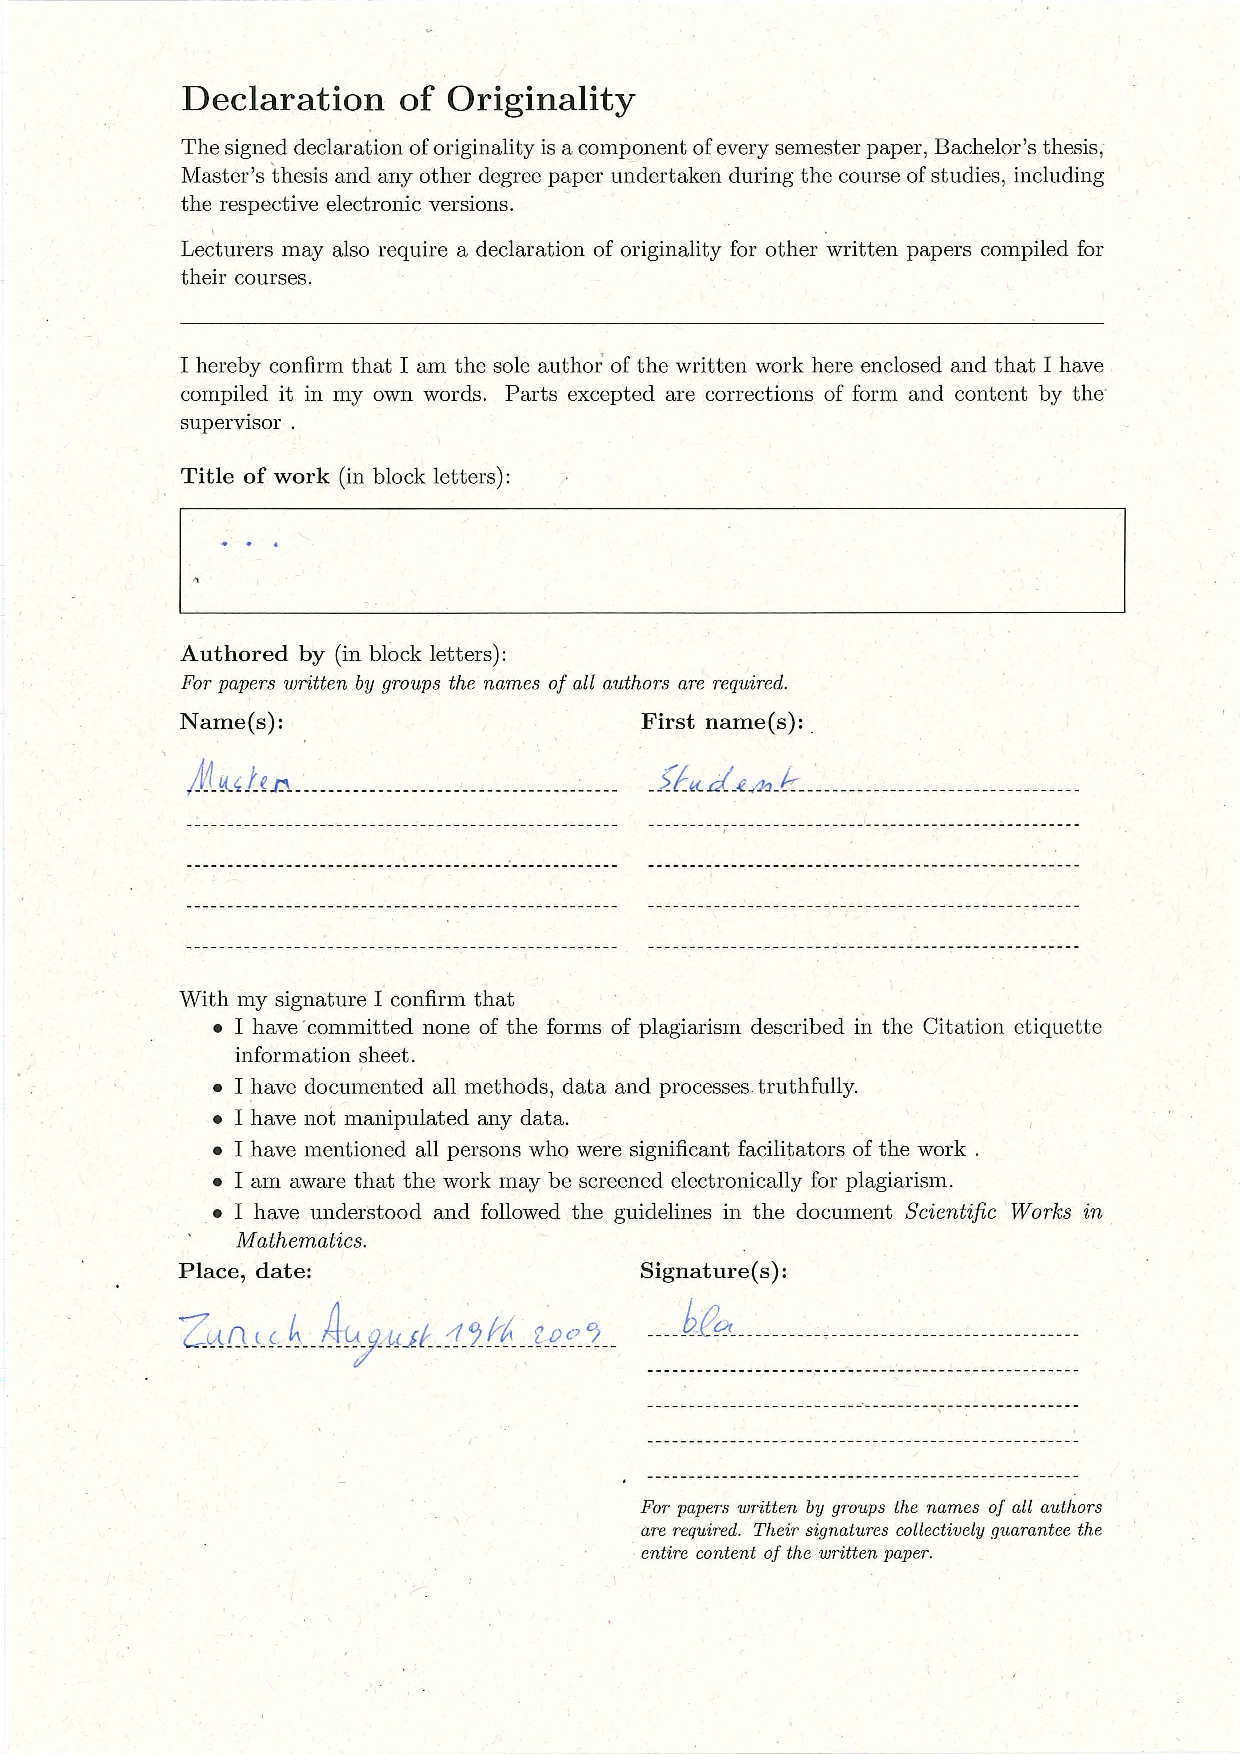
\includepdf[pages={-}, frame=true,scale=1]{confirmation-originality-scan.pdf}
\end{document}

%%% Local Variables:
%%% mode: latex
%%% TeX-master: "MasterThesisSfS"
%%% End:
